\chapter{Method}

\section{Description of The Datasets} \label{sec:datasets}

Since the different \acrshort{ml} models require different types of input data the, datasets have been divided into two main categories: 
The peak-value datasets and the time-series datasets. \bigskip

\subsection{Time-series Datasets} \label{sec:ts_dsets}

\begin{table*}[h]
    \centering
    \ra{1.3}
    \begin{tabular}{ rlr }
        \toprule
        Nr & Input variables   & Shape \\
        \midrule
        1  & Single \acrshort{rls} curves & $(3600,1)$ \\
        2  & \acrshort{rls} curves        & $(200,18)$ \\
        3  & \acrshort{gls} curves        & $(200,3)$  \\
        4  & Strain curves                & $(200,21)$ \\
        \bottomrule
    \end{tabular}
    \caption{Time-series datasets. The ''Shape'' parameter is indicates: (Number of objects in the dataset, Number of curves used to represent each individual object). The curve length is not included in the shape parameter because it differs for different curves.}
    \label{tab:ts_dsets}
\end{table*}

Table \ref{tab:ts_dsets} shows the different time-series datasets that will be used. 
All the datasets except \textit{Single \acrshort{rls} curves} will be used to predict whether or not the patient is diagnosed, and whether the patient has heart failure. Recall that the different diagnosises are described in section REFERENCE, and there occurance rate are illustrated in figure \ref{fig:hf_ind_dist}.\textit{Single \acrshort{rls} curves} will be used to predict the segment indications shown in figure \ref{fig:segm_label_dist} and described in section REFERENCE. The point of classifying individual segments of a patients left ventricle is that if a single segment is found to be \textit{not normal}, this would also mean that the patient can be considered as \textit{not healthy}. As mentioned in the description of table \ref{tab:ts_dsets} the ''Shape'' parameter shows how many objects each dataset has, and how many curves are associated to each object. Since each ultrasound examination takes ultrasound inspections from three views (four chamber, two chamber, and APLAX chamber), each patient has three views to estimate a \acrshort{gls} curve from. Since each \acrshort{gls} curve, also can be divided into six \acrshort{rls} curves, there is a total of 21 strain curves per patient. Since each patient has 18 \acrshort{rls} curves, there are $18 \times 200 = 3600$ curves that make up dataset number 1. For datasets two to three it will also be experimented with wether using data from a single view performs better than data from all views. For dataset two that means that the number of curves used to represent an object will be either 6 or 18, for dataset three it will be either 1 or 3 curves and for dataset four patients will be represented with either 7 or 21 curves. Both the \acrshort{ann}, and the \acrshort{tsc} model are applied on the datasets listed in table \ref{tab:ts_dsets}. \bigskip

\subsection{Peak-value Datasets}

\begin{table*}[h]
    \centering
    \ra{1.3}
    \begin{tabular}{ rlr }
        \toprule
        Nr & Input variables                                           & Shape \\
        \midrule                              
        1  & Peak systolic \acrshort{rls} values                       & $(200,18)$ \\
        2  & Peak systolic \acrshort{gls} values                       & $(200,3)$  \\
        3  & Peak systolic strain values                               & $(200,21)$ \\
        4  & Peak systolic \acrshort{rls}, and \acrshort{ef} values    & $(200,19)$ \\
        5  & Peak systolic \acrshort{gls}, and \acrshort{ef} values    & $(200,4)$  \\
        6  & Peak systolic strain, and \acrshort{ef} values            & $(200,22)$ \\
        \bottomrule
    \end{tabular}
    \caption{Peak-value datasets. The ''Shape'' parameter is indicates: (Number of objects in the dataset, Number of dimensions used to represent each individual object).}
    \label{tab:pv_dsets}
\end{table*}

Table \ref{tab:pv_dsets} shows the different peak-value datasets. All the datasets will be used to predict the diagnosis of patients, and whether the patient has heart failure. Single peak systolic \acrshort{rls} values were not considered suited for \acrshort{pvc} or \acrshort{pvsc} models to predict segment indication, because the best model one can hope for from a one dimensional point-value dataset is a form of threshold classifier. The reason that there are more peak-value datasets than there are time-series datasets, is that the peak-value version of three datasets in table \ref{tab:ts_dsets} have been combined with \acrshort{ef} to determine whether a combination of peak systolic strain, and \acrshort{ef} can have a higher predictive power than strain alone.

\section{Clustering} \label{sec:meth_clust}

The implementations of the two clustering models that are applied in this work are described together in the same section because conceptually, they are almost identical. It is only the method used to measure dissimilarity that separates the \acrshort{pvc} and \acrshort{tsc} models. The general implementation of the clustering models is illustrated in figure \ref{fig:clust_flow}. Time-series datasets are preprocessed before dissimilarity measurement, peak-value datasets are not. In the coming subsections the processes in each of the boxes in the flow diagram will be expanded upon.

\begin{figure}
    \centering
    \tikzstyle{IO}    = [draw, ellipse,fill=red!20, minimum height=2em]
\tikzstyle{block} = [rectangle, draw, fill=blue!20, text width=7em, text centered, rounded corners, minimum height=2em]
\tikzstyle{evl}   = [rectangle, draw, fill=green!20, text width=7em, text centered, minimum height=2em]
\tikzstyle{arrow} = [thin,->,>=stealth]

\begin{tikzpicture}
% Shapes
\node (input)   [IO] {Input data};
\node (preproc) [block, node distance=1.5cm, below of=input]   {Preprocessing};
\node (diss)    [block, node distance=1.5cm, below of=preproc] {Dissimilarity measurement};
\node (clust)   [block, node distance=2cm, below of=diss]  {Hierarchical Agglomerative Clustering};
\node (output)  [IO,    node distance=2cm, below of=clust] {Cluster assignments};
\node (ari)     [evl,   node distance=1.5cm, below of=output, xshift=-3cm] {ARI};
\node (dor)     [evl,   node distance=2.1cm, below of=output, xshift=3cm] {TP, TN, FP and FN};

% Arrows
\draw [arrow] (input)   --node[anchor=west] {}                     (preproc);
\draw [arrow] (preproc) --node[anchor=west] {Processed data}       (diss);
\draw [arrow] (diss)    --node[anchor=west] {Dissimilarity matrix} (clust);
\draw [arrow] (clust)   --node[anchor=west] {}                     (output);
\draw [arrow] (output)  --node[anchor=east] {$2 \rightarrow 9$}    (ari);
\draw [arrow] (output)  --node[anchor=west] {2}                    (dor);
\end{tikzpicture}

    \caption{A flow diagram to give an overview of how the \acrshort{pvc} and \acrshort{tsc} models are implemented and evaluated.}
    \label{fig:clust_flow}
\end{figure}

\clearpage

\subsection{Time-series Preprocessing}
Preprocessing of the time series is done because it is known that the \acrshort{dtw} distance is sensitive to absolute difference, and offsets of time series. In addition to clustering the longitudinal strain time series without preprocessing three forms of preprocessing were tested to see whether they could improve the predictive performance of the clustering algorithm: Normalization, scaling and Z-score normalization. The normalized version of a time series ($\{x_t\}_N$) is calculated by equation \eqref{eq:ts_norm}. The smallest recorded value in the time series ($\mathrm{min}\{x_t\}$) is subtracted from the time series ($\{x_t\}$), then the time series is divided by the difference between the highest recorded value ($\mathrm{max}\{x_t\}$), and lowest recorded value in the time series.

\begin{equation}
    \{x_t\}_N = \frac{\{x_t\} - \mathrm{min}\{x_t\}}{\mathrm{max}\{x_t\} - \mathrm{min}\{x_t\}}
    \label{eq:ts_norm}
\end{equation}

The ''scaled'' version of a times is calculated in a similar fashion. Scaling can be considered as normalizing a time series with regard to the highest, and lowest recorded values of the entire set of time series it is being compared to. If one lets $\{ \left \{ x_t \} \right \}$ represent the set of time series to be scaled, $\mathrm{min}\{ \left \{ x_t \} \right \}$ represent the smallest recorded value in the entire set of time series and $\mathrm{max}\{ \left \{ x_t \} \right \}$ represent the highest recorded value in the set of time series, the scaled version of a time series ($\{x_t\}_S$) is given by eqation \eqref{eq:ts_scale}.

\begin{equation}
    \{x_t\}_S = \frac{\{x_t\} - \mathrm{min}\{ \left \{ x_t \} \right \}}{\mathrm{max}\{ \left \{ x_t \} \right \} - \mathrm{min}\{ \left \{ x_t \} \right \}}
    \label{eq:ts_scale}
\end{equation}

The Z-score normalization is done by transforming each observation of a time series to it's Z-score. The Z-score of an individual time-series observation is calculated by subracting the expected value of the time series, and dividing by the standard deviation. The unbiased estimators used to calculate the expected value, and standard deviation of a time series are given in equations \eqref{eq:ev_est}, and \eqref{eq:std_est} respectively. The Z-score normalized version of a time series ($\{x_t\}_Z$) is calculated using equation \eqref{eq:ts_zscn}

\begin{equation}
    \hat{\mu} = \frac{1}{n} \sum^n_{t = 1} x_t
    \label{eq:ev_est}
\end{equation}

\begin{equation}
    \hat{\sigma} = \sqrt{\frac{1}{n - 1} \sum^n_{t = 1} (x_t - \hat{\mu})^2}
    \label{eq:std_est}
\end{equation}

\begin{equation}
    \{x_t\}_Z = \frac{\{x_t\} - \hat{\mu}}{\hat{\sigma}}
    \label{eq:ts_zscn}
\end{equation}

Figure \ref{fig:preproc} illustrates how the different preprocessing methods work on the \acrshort{4ch} \acrshort{gls} curves of four random patients. By comparing \ref{fig:preproc}a and \ref{fig:preproc}d one can see that scaling preserves both the relative offsets and relative size differences between the curves. From \ref{fig:preproc}b one can see that though normalization preserves the offsets of the curves, the relative sizes are not. From \ref{fig:preproc}c one can see that Z-score normalization preserves the offsets of the curves, the relative sizes are only preserved to a certain extent. In addition, the normalized, and scaled curves are constricted between 0 and 1, while the Z-score normalized curves are not.  

\begin{figure}
    \centering
    %% Creator: Matplotlib, PGF backend
%%
%% To include the figure in your LaTeX document, write
%%   \input{<filename>.pgf}
%%
%% Make sure the required packages are loaded in your preamble
%%   \usepackage{pgf}
%%
%% Figures using additional raster images can only be included by \input if
%% they are in the same directory as the main LaTeX file. For loading figures
%% from other directories you can use the `import` package
%%   \usepackage{import}
%% and then include the figures with
%%   \import{<path to file>}{<filename>.pgf}
%%
%% Matplotlib used the following preamble
%%
\begingroup%
\makeatletter%
\begin{pgfpicture}%
\pgfpathrectangle{\pgfpointorigin}{\pgfqpoint{6.400000in}{6.400000in}}%
\pgfusepath{use as bounding box, clip}%
\begin{pgfscope}%
\pgfsetbuttcap%
\pgfsetmiterjoin%
\definecolor{currentfill}{rgb}{1.000000,1.000000,1.000000}%
\pgfsetfillcolor{currentfill}%
\pgfsetlinewidth{0.000000pt}%
\definecolor{currentstroke}{rgb}{1.000000,1.000000,1.000000}%
\pgfsetstrokecolor{currentstroke}%
\pgfsetdash{}{0pt}%
\pgfpathmoveto{\pgfqpoint{0.000000in}{0.000000in}}%
\pgfpathlineto{\pgfqpoint{6.400000in}{0.000000in}}%
\pgfpathlineto{\pgfqpoint{6.400000in}{6.400000in}}%
\pgfpathlineto{\pgfqpoint{0.000000in}{6.400000in}}%
\pgfpathclose%
\pgfusepath{fill}%
\end{pgfscope}%
\begin{pgfscope}%
\pgfsetbuttcap%
\pgfsetmiterjoin%
\definecolor{currentfill}{rgb}{1.000000,1.000000,1.000000}%
\pgfsetfillcolor{currentfill}%
\pgfsetlinewidth{0.000000pt}%
\definecolor{currentstroke}{rgb}{0.000000,0.000000,0.000000}%
\pgfsetstrokecolor{currentstroke}%
\pgfsetstrokeopacity{0.000000}%
\pgfsetdash{}{0pt}%
\pgfpathmoveto{\pgfqpoint{0.693748in}{3.520370in}}%
\pgfpathlineto{\pgfqpoint{3.269001in}{3.520370in}}%
\pgfpathlineto{\pgfqpoint{3.269001in}{6.091667in}}%
\pgfpathlineto{\pgfqpoint{0.693748in}{6.091667in}}%
\pgfpathclose%
\pgfusepath{fill}%
\end{pgfscope}%
\begin{pgfscope}%
\pgfsetbuttcap%
\pgfsetroundjoin%
\definecolor{currentfill}{rgb}{0.000000,0.000000,0.000000}%
\pgfsetfillcolor{currentfill}%
\pgfsetlinewidth{0.803000pt}%
\definecolor{currentstroke}{rgb}{0.000000,0.000000,0.000000}%
\pgfsetstrokecolor{currentstroke}%
\pgfsetdash{}{0pt}%
\pgfsys@defobject{currentmarker}{\pgfqpoint{0.000000in}{-0.048611in}}{\pgfqpoint{0.000000in}{0.000000in}}{%
\pgfpathmoveto{\pgfqpoint{0.000000in}{0.000000in}}%
\pgfpathlineto{\pgfqpoint{0.000000in}{-0.048611in}}%
\pgfusepath{stroke,fill}%
}%
\begin{pgfscope}%
\pgfsys@transformshift{0.810805in}{3.520370in}%
\pgfsys@useobject{currentmarker}{}%
\end{pgfscope}%
\end{pgfscope}%
\begin{pgfscope}%
\definecolor{textcolor}{rgb}{0.000000,0.000000,0.000000}%
\pgfsetstrokecolor{textcolor}%
\pgfsetfillcolor{textcolor}%
\pgftext[x=0.810805in,y=3.423148in,,top]{\color{textcolor}\rmfamily\fontsize{12.000000}{14.400000}\selectfont \(\displaystyle 0\)}%
\end{pgfscope}%
\begin{pgfscope}%
\pgfsetbuttcap%
\pgfsetroundjoin%
\definecolor{currentfill}{rgb}{0.000000,0.000000,0.000000}%
\pgfsetfillcolor{currentfill}%
\pgfsetlinewidth{0.803000pt}%
\definecolor{currentstroke}{rgb}{0.000000,0.000000,0.000000}%
\pgfsetstrokecolor{currentstroke}%
\pgfsetdash{}{0pt}%
\pgfsys@defobject{currentmarker}{\pgfqpoint{0.000000in}{-0.048611in}}{\pgfqpoint{0.000000in}{0.000000in}}{%
\pgfpathmoveto{\pgfqpoint{0.000000in}{0.000000in}}%
\pgfpathlineto{\pgfqpoint{0.000000in}{-0.048611in}}%
\pgfusepath{stroke,fill}%
}%
\begin{pgfscope}%
\pgfsys@transformshift{1.348998in}{3.520370in}%
\pgfsys@useobject{currentmarker}{}%
\end{pgfscope}%
\end{pgfscope}%
\begin{pgfscope}%
\definecolor{textcolor}{rgb}{0.000000,0.000000,0.000000}%
\pgfsetstrokecolor{textcolor}%
\pgfsetfillcolor{textcolor}%
\pgftext[x=1.348998in,y=3.423148in,,top]{\color{textcolor}\rmfamily\fontsize{12.000000}{14.400000}\selectfont \(\displaystyle 20\)}%
\end{pgfscope}%
\begin{pgfscope}%
\pgfsetbuttcap%
\pgfsetroundjoin%
\definecolor{currentfill}{rgb}{0.000000,0.000000,0.000000}%
\pgfsetfillcolor{currentfill}%
\pgfsetlinewidth{0.803000pt}%
\definecolor{currentstroke}{rgb}{0.000000,0.000000,0.000000}%
\pgfsetstrokecolor{currentstroke}%
\pgfsetdash{}{0pt}%
\pgfsys@defobject{currentmarker}{\pgfqpoint{0.000000in}{-0.048611in}}{\pgfqpoint{0.000000in}{0.000000in}}{%
\pgfpathmoveto{\pgfqpoint{0.000000in}{0.000000in}}%
\pgfpathlineto{\pgfqpoint{0.000000in}{-0.048611in}}%
\pgfusepath{stroke,fill}%
}%
\begin{pgfscope}%
\pgfsys@transformshift{1.887191in}{3.520370in}%
\pgfsys@useobject{currentmarker}{}%
\end{pgfscope}%
\end{pgfscope}%
\begin{pgfscope}%
\definecolor{textcolor}{rgb}{0.000000,0.000000,0.000000}%
\pgfsetstrokecolor{textcolor}%
\pgfsetfillcolor{textcolor}%
\pgftext[x=1.887191in,y=3.423148in,,top]{\color{textcolor}\rmfamily\fontsize{12.000000}{14.400000}\selectfont \(\displaystyle 40\)}%
\end{pgfscope}%
\begin{pgfscope}%
\pgfsetbuttcap%
\pgfsetroundjoin%
\definecolor{currentfill}{rgb}{0.000000,0.000000,0.000000}%
\pgfsetfillcolor{currentfill}%
\pgfsetlinewidth{0.803000pt}%
\definecolor{currentstroke}{rgb}{0.000000,0.000000,0.000000}%
\pgfsetstrokecolor{currentstroke}%
\pgfsetdash{}{0pt}%
\pgfsys@defobject{currentmarker}{\pgfqpoint{0.000000in}{-0.048611in}}{\pgfqpoint{0.000000in}{0.000000in}}{%
\pgfpathmoveto{\pgfqpoint{0.000000in}{0.000000in}}%
\pgfpathlineto{\pgfqpoint{0.000000in}{-0.048611in}}%
\pgfusepath{stroke,fill}%
}%
\begin{pgfscope}%
\pgfsys@transformshift{2.425384in}{3.520370in}%
\pgfsys@useobject{currentmarker}{}%
\end{pgfscope}%
\end{pgfscope}%
\begin{pgfscope}%
\definecolor{textcolor}{rgb}{0.000000,0.000000,0.000000}%
\pgfsetstrokecolor{textcolor}%
\pgfsetfillcolor{textcolor}%
\pgftext[x=2.425384in,y=3.423148in,,top]{\color{textcolor}\rmfamily\fontsize{12.000000}{14.400000}\selectfont \(\displaystyle 60\)}%
\end{pgfscope}%
\begin{pgfscope}%
\pgfsetbuttcap%
\pgfsetroundjoin%
\definecolor{currentfill}{rgb}{0.000000,0.000000,0.000000}%
\pgfsetfillcolor{currentfill}%
\pgfsetlinewidth{0.803000pt}%
\definecolor{currentstroke}{rgb}{0.000000,0.000000,0.000000}%
\pgfsetstrokecolor{currentstroke}%
\pgfsetdash{}{0pt}%
\pgfsys@defobject{currentmarker}{\pgfqpoint{0.000000in}{-0.048611in}}{\pgfqpoint{0.000000in}{0.000000in}}{%
\pgfpathmoveto{\pgfqpoint{0.000000in}{0.000000in}}%
\pgfpathlineto{\pgfqpoint{0.000000in}{-0.048611in}}%
\pgfusepath{stroke,fill}%
}%
\begin{pgfscope}%
\pgfsys@transformshift{2.963576in}{3.520370in}%
\pgfsys@useobject{currentmarker}{}%
\end{pgfscope}%
\end{pgfscope}%
\begin{pgfscope}%
\definecolor{textcolor}{rgb}{0.000000,0.000000,0.000000}%
\pgfsetstrokecolor{textcolor}%
\pgfsetfillcolor{textcolor}%
\pgftext[x=2.963576in,y=3.423148in,,top]{\color{textcolor}\rmfamily\fontsize{12.000000}{14.400000}\selectfont \(\displaystyle 80\)}%
\end{pgfscope}%
\begin{pgfscope}%
\pgfsetbuttcap%
\pgfsetroundjoin%
\definecolor{currentfill}{rgb}{0.000000,0.000000,0.000000}%
\pgfsetfillcolor{currentfill}%
\pgfsetlinewidth{0.803000pt}%
\definecolor{currentstroke}{rgb}{0.000000,0.000000,0.000000}%
\pgfsetstrokecolor{currentstroke}%
\pgfsetdash{}{0pt}%
\pgfsys@defobject{currentmarker}{\pgfqpoint{-0.048611in}{0.000000in}}{\pgfqpoint{0.000000in}{0.000000in}}{%
\pgfpathmoveto{\pgfqpoint{0.000000in}{0.000000in}}%
\pgfpathlineto{\pgfqpoint{-0.048611in}{0.000000in}}%
\pgfusepath{stroke,fill}%
}%
\begin{pgfscope}%
\pgfsys@transformshift{0.693748in}{3.698853in}%
\pgfsys@useobject{currentmarker}{}%
\end{pgfscope}%
\end{pgfscope}%
\begin{pgfscope}%
\definecolor{textcolor}{rgb}{0.000000,0.000000,0.000000}%
\pgfsetstrokecolor{textcolor}%
\pgfsetfillcolor{textcolor}%
\pgftext[x=0.303703in,y=3.640983in,left,base]{\color{textcolor}\rmfamily\fontsize{12.000000}{14.400000}\selectfont \(\displaystyle -15\)}%
\end{pgfscope}%
\begin{pgfscope}%
\pgfsetbuttcap%
\pgfsetroundjoin%
\definecolor{currentfill}{rgb}{0.000000,0.000000,0.000000}%
\pgfsetfillcolor{currentfill}%
\pgfsetlinewidth{0.803000pt}%
\definecolor{currentstroke}{rgb}{0.000000,0.000000,0.000000}%
\pgfsetstrokecolor{currentstroke}%
\pgfsetdash{}{0pt}%
\pgfsys@defobject{currentmarker}{\pgfqpoint{-0.048611in}{0.000000in}}{\pgfqpoint{0.000000in}{0.000000in}}{%
\pgfpathmoveto{\pgfqpoint{0.000000in}{0.000000in}}%
\pgfpathlineto{\pgfqpoint{-0.048611in}{0.000000in}}%
\pgfusepath{stroke,fill}%
}%
\begin{pgfscope}%
\pgfsys@transformshift{0.693748in}{4.429378in}%
\pgfsys@useobject{currentmarker}{}%
\end{pgfscope}%
\end{pgfscope}%
\begin{pgfscope}%
\definecolor{textcolor}{rgb}{0.000000,0.000000,0.000000}%
\pgfsetstrokecolor{textcolor}%
\pgfsetfillcolor{textcolor}%
\pgftext[x=0.303703in,y=4.371508in,left,base]{\color{textcolor}\rmfamily\fontsize{12.000000}{14.400000}\selectfont \(\displaystyle -10\)}%
\end{pgfscope}%
\begin{pgfscope}%
\pgfsetbuttcap%
\pgfsetroundjoin%
\definecolor{currentfill}{rgb}{0.000000,0.000000,0.000000}%
\pgfsetfillcolor{currentfill}%
\pgfsetlinewidth{0.803000pt}%
\definecolor{currentstroke}{rgb}{0.000000,0.000000,0.000000}%
\pgfsetstrokecolor{currentstroke}%
\pgfsetdash{}{0pt}%
\pgfsys@defobject{currentmarker}{\pgfqpoint{-0.048611in}{0.000000in}}{\pgfqpoint{0.000000in}{0.000000in}}{%
\pgfpathmoveto{\pgfqpoint{0.000000in}{0.000000in}}%
\pgfpathlineto{\pgfqpoint{-0.048611in}{0.000000in}}%
\pgfusepath{stroke,fill}%
}%
\begin{pgfscope}%
\pgfsys@transformshift{0.693748in}{5.159903in}%
\pgfsys@useobject{currentmarker}{}%
\end{pgfscope}%
\end{pgfscope}%
\begin{pgfscope}%
\definecolor{textcolor}{rgb}{0.000000,0.000000,0.000000}%
\pgfsetstrokecolor{textcolor}%
\pgfsetfillcolor{textcolor}%
\pgftext[x=0.385299in,y=5.102033in,left,base]{\color{textcolor}\rmfamily\fontsize{12.000000}{14.400000}\selectfont \(\displaystyle -5\)}%
\end{pgfscope}%
\begin{pgfscope}%
\pgfsetbuttcap%
\pgfsetroundjoin%
\definecolor{currentfill}{rgb}{0.000000,0.000000,0.000000}%
\pgfsetfillcolor{currentfill}%
\pgfsetlinewidth{0.803000pt}%
\definecolor{currentstroke}{rgb}{0.000000,0.000000,0.000000}%
\pgfsetstrokecolor{currentstroke}%
\pgfsetdash{}{0pt}%
\pgfsys@defobject{currentmarker}{\pgfqpoint{-0.048611in}{0.000000in}}{\pgfqpoint{0.000000in}{0.000000in}}{%
\pgfpathmoveto{\pgfqpoint{0.000000in}{0.000000in}}%
\pgfpathlineto{\pgfqpoint{-0.048611in}{0.000000in}}%
\pgfusepath{stroke,fill}%
}%
\begin{pgfscope}%
\pgfsys@transformshift{0.693748in}{5.890428in}%
\pgfsys@useobject{currentmarker}{}%
\end{pgfscope}%
\end{pgfscope}%
\begin{pgfscope}%
\definecolor{textcolor}{rgb}{0.000000,0.000000,0.000000}%
\pgfsetstrokecolor{textcolor}%
\pgfsetfillcolor{textcolor}%
\pgftext[x=0.514929in,y=5.832558in,left,base]{\color{textcolor}\rmfamily\fontsize{12.000000}{14.400000}\selectfont \(\displaystyle 0\)}%
\end{pgfscope}%
\begin{pgfscope}%
\definecolor{textcolor}{rgb}{0.000000,0.000000,0.000000}%
\pgfsetstrokecolor{textcolor}%
\pgfsetfillcolor{textcolor}%
\pgftext[x=0.248148in,y=4.806018in,,bottom,rotate=90.000000]{\color{textcolor}\rmfamily\fontsize{12.000000}{14.400000}\selectfont Strain}%
\end{pgfscope}%
\begin{pgfscope}%
\pgfpathrectangle{\pgfqpoint{0.693748in}{3.520370in}}{\pgfqpoint{2.575253in}{2.571297in}}%
\pgfusepath{clip}%
\pgfsetrectcap%
\pgfsetroundjoin%
\pgfsetlinewidth{1.505625pt}%
\definecolor{currentstroke}{rgb}{0.121569,0.466667,0.705882}%
\pgfsetstrokecolor{currentstroke}%
\pgfsetdash{}{0pt}%
\pgfpathmoveto{\pgfqpoint{0.810805in}{4.909606in}}%
\pgfpathlineto{\pgfqpoint{0.837715in}{5.009442in}}%
\pgfpathlineto{\pgfqpoint{0.864624in}{5.137607in}}%
\pgfpathlineto{\pgfqpoint{0.891534in}{5.303902in}}%
\pgfpathlineto{\pgfqpoint{0.918444in}{5.494865in}}%
\pgfpathlineto{\pgfqpoint{0.945353in}{5.679574in}}%
\pgfpathlineto{\pgfqpoint{0.972263in}{5.823424in}}%
\pgfpathlineto{\pgfqpoint{0.999173in}{5.908722in}}%
\pgfpathlineto{\pgfqpoint{1.026082in}{5.942091in}}%
\pgfpathlineto{\pgfqpoint{1.052992in}{5.941784in}}%
\pgfpathlineto{\pgfqpoint{1.079901in}{5.924005in}}%
\pgfpathlineto{\pgfqpoint{1.106811in}{5.902753in}}%
\pgfpathlineto{\pgfqpoint{1.133721in}{5.890428in}}%
\pgfpathlineto{\pgfqpoint{1.160630in}{5.892809in}}%
\pgfpathlineto{\pgfqpoint{1.187540in}{5.904969in}}%
\pgfpathlineto{\pgfqpoint{1.214450in}{5.911575in}}%
\pgfpathlineto{\pgfqpoint{1.241359in}{5.894517in}}%
\pgfpathlineto{\pgfqpoint{1.268269in}{5.844482in}}%
\pgfpathlineto{\pgfqpoint{1.295179in}{5.764338in}}%
\pgfpathlineto{\pgfqpoint{1.322088in}{5.662964in}}%
\pgfpathlineto{\pgfqpoint{1.348998in}{5.550368in}}%
\pgfpathlineto{\pgfqpoint{1.375908in}{5.435144in}}%
\pgfpathlineto{\pgfqpoint{1.402817in}{5.321923in}}%
\pgfpathlineto{\pgfqpoint{1.429727in}{5.210320in}}%
\pgfpathlineto{\pgfqpoint{1.456636in}{5.097667in}}%
\pgfpathlineto{\pgfqpoint{1.483546in}{4.983696in}}%
\pgfpathlineto{\pgfqpoint{1.510456in}{4.871054in}}%
\pgfpathlineto{\pgfqpoint{1.537365in}{4.761590in}}%
\pgfpathlineto{\pgfqpoint{1.564275in}{4.655328in}}%
\pgfpathlineto{\pgfqpoint{1.591185in}{4.553648in}}%
\pgfpathlineto{\pgfqpoint{1.618094in}{4.458228in}}%
\pgfpathlineto{\pgfqpoint{1.645004in}{4.370831in}}%
\pgfpathlineto{\pgfqpoint{1.671914in}{4.293544in}}%
\pgfpathlineto{\pgfqpoint{1.698823in}{4.229239in}}%
\pgfpathlineto{\pgfqpoint{1.725733in}{4.180946in}}%
\pgfpathlineto{\pgfqpoint{1.752643in}{4.150458in}}%
\pgfpathlineto{\pgfqpoint{1.779552in}{4.137840in}}%
\pgfpathlineto{\pgfqpoint{1.806462in}{4.141755in}}%
\pgfpathlineto{\pgfqpoint{1.833371in}{4.158713in}}%
\pgfpathlineto{\pgfqpoint{1.860281in}{4.179740in}}%
\pgfpathlineto{\pgfqpoint{1.887191in}{4.191514in}}%
\pgfpathlineto{\pgfqpoint{1.914100in}{4.185875in}}%
\pgfpathlineto{\pgfqpoint{1.941010in}{4.166779in}}%
\pgfpathlineto{\pgfqpoint{1.967920in}{4.148212in}}%
\pgfpathlineto{\pgfqpoint{1.994829in}{4.144751in}}%
\pgfpathlineto{\pgfqpoint{2.021739in}{4.164043in}}%
\pgfpathlineto{\pgfqpoint{2.048649in}{4.205078in}}%
\pgfpathlineto{\pgfqpoint{2.075558in}{4.259021in}}%
\pgfpathlineto{\pgfqpoint{2.102468in}{4.314952in}}%
\pgfpathlineto{\pgfqpoint{2.129378in}{4.366553in}}%
\pgfpathlineto{\pgfqpoint{2.156287in}{4.413264in}}%
\pgfpathlineto{\pgfqpoint{2.183197in}{4.457854in}}%
\pgfpathlineto{\pgfqpoint{2.210106in}{4.503348in}}%
\pgfpathlineto{\pgfqpoint{2.237016in}{4.551042in}}%
\pgfpathlineto{\pgfqpoint{2.263926in}{4.600086in}}%
\pgfpathlineto{\pgfqpoint{2.290835in}{4.648629in}}%
\pgfpathlineto{\pgfqpoint{2.317745in}{4.694911in}}%
\pgfpathlineto{\pgfqpoint{2.344655in}{4.737850in}}%
\pgfpathlineto{\pgfqpoint{2.371564in}{4.777064in}}%
\pgfpathlineto{\pgfqpoint{2.398474in}{4.813378in}}%
\pgfpathlineto{\pgfqpoint{2.425384in}{4.854171in}}%
\pgfpathlineto{\pgfqpoint{2.452293in}{4.917717in}}%
\pgfpathlineto{\pgfqpoint{2.479203in}{5.026686in}}%
\pgfpathlineto{\pgfqpoint{2.506113in}{5.191696in}}%
\pgfpathlineto{\pgfqpoint{2.533022in}{5.398009in}}%
\pgfpathlineto{\pgfqpoint{2.559932in}{5.608273in}}%
\pgfpathlineto{\pgfqpoint{2.586841in}{5.780355in}}%
\pgfpathlineto{\pgfqpoint{2.613751in}{5.889180in}}%
\pgfpathlineto{\pgfqpoint{2.640661in}{5.936001in}}%
\pgfpathlineto{\pgfqpoint{2.667570in}{5.939834in}}%
\pgfpathlineto{\pgfqpoint{2.694480in}{5.922220in}}%
\pgfpathlineto{\pgfqpoint{2.721390in}{5.901167in}}%
\pgfpathlineto{\pgfqpoint{2.748299in}{5.890428in}}%
\pgfpathlineto{\pgfqpoint{2.775209in}{5.896020in}}%
\pgfpathlineto{\pgfqpoint{2.802119in}{5.911628in}}%
\pgfpathlineto{\pgfqpoint{2.829028in}{5.921483in}}%
\pgfpathlineto{\pgfqpoint{2.855938in}{5.910098in}}%
\pgfpathlineto{\pgfqpoint{2.882848in}{5.868840in}}%
\pgfpathlineto{\pgfqpoint{2.909757in}{5.797889in}}%
\pgfpathlineto{\pgfqpoint{2.936667in}{5.703420in}}%
\pgfpathlineto{\pgfqpoint{2.963576in}{5.593517in}}%
\pgfpathlineto{\pgfqpoint{2.990486in}{5.477352in}}%
\pgfpathlineto{\pgfqpoint{3.017396in}{5.362659in}}%
\pgfpathlineto{\pgfqpoint{3.044305in}{5.252797in}}%
\pgfpathlineto{\pgfqpoint{3.071215in}{5.146348in}}%
\pgfusepath{stroke}%
\end{pgfscope}%
\begin{pgfscope}%
\pgfpathrectangle{\pgfqpoint{0.693748in}{3.520370in}}{\pgfqpoint{2.575253in}{2.571297in}}%
\pgfusepath{clip}%
\pgfsetrectcap%
\pgfsetroundjoin%
\pgfsetlinewidth{1.505625pt}%
\definecolor{currentstroke}{rgb}{1.000000,0.498039,0.054902}%
\pgfsetstrokecolor{currentstroke}%
\pgfsetdash{}{0pt}%
\pgfpathmoveto{\pgfqpoint{0.810805in}{5.343090in}}%
\pgfpathlineto{\pgfqpoint{0.837715in}{5.348397in}}%
\pgfpathlineto{\pgfqpoint{0.864624in}{5.362262in}}%
\pgfpathlineto{\pgfqpoint{0.891534in}{5.397276in}}%
\pgfpathlineto{\pgfqpoint{0.918444in}{5.465259in}}%
\pgfpathlineto{\pgfqpoint{0.945353in}{5.566059in}}%
\pgfpathlineto{\pgfqpoint{0.972263in}{5.685322in}}%
\pgfpathlineto{\pgfqpoint{0.999173in}{5.796150in}}%
\pgfpathlineto{\pgfqpoint{1.026082in}{5.875747in}}%
\pgfpathlineto{\pgfqpoint{1.052992in}{5.913938in}}%
\pgfpathlineto{\pgfqpoint{1.079901in}{5.914767in}}%
\pgfpathlineto{\pgfqpoint{1.106811in}{5.890428in}}%
\pgfpathlineto{\pgfqpoint{1.133721in}{5.858131in}}%
\pgfpathlineto{\pgfqpoint{1.160630in}{5.828283in}}%
\pgfpathlineto{\pgfqpoint{1.187540in}{5.793359in}}%
\pgfpathlineto{\pgfqpoint{1.214450in}{5.733937in}}%
\pgfpathlineto{\pgfqpoint{1.241359in}{5.637632in}}%
\pgfpathlineto{\pgfqpoint{1.268269in}{5.514021in}}%
\pgfpathlineto{\pgfqpoint{1.295179in}{5.386128in}}%
\pgfpathlineto{\pgfqpoint{1.322088in}{5.273123in}}%
\pgfpathlineto{\pgfqpoint{1.348998in}{5.181896in}}%
\pgfpathlineto{\pgfqpoint{1.375908in}{5.102292in}}%
\pgfpathlineto{\pgfqpoint{1.402817in}{5.014035in}}%
\pgfpathlineto{\pgfqpoint{1.429727in}{4.904134in}}%
\pgfpathlineto{\pgfqpoint{1.456636in}{4.777201in}}%
\pgfpathlineto{\pgfqpoint{1.483546in}{4.646831in}}%
\pgfpathlineto{\pgfqpoint{1.510456in}{4.526044in}}%
\pgfpathlineto{\pgfqpoint{1.537365in}{4.421820in}}%
\pgfpathlineto{\pgfqpoint{1.564275in}{4.339871in}}%
\pgfpathlineto{\pgfqpoint{1.591185in}{4.284714in}}%
\pgfpathlineto{\pgfqpoint{1.618094in}{4.258985in}}%
\pgfpathlineto{\pgfqpoint{1.645004in}{4.260839in}}%
\pgfpathlineto{\pgfqpoint{1.671914in}{4.283573in}}%
\pgfpathlineto{\pgfqpoint{1.698823in}{4.321151in}}%
\pgfpathlineto{\pgfqpoint{1.725733in}{4.372884in}}%
\pgfpathlineto{\pgfqpoint{1.752643in}{4.442895in}}%
\pgfpathlineto{\pgfqpoint{1.779552in}{4.530497in}}%
\pgfpathlineto{\pgfqpoint{1.806462in}{4.622801in}}%
\pgfpathlineto{\pgfqpoint{1.833371in}{4.705210in}}%
\pgfpathlineto{\pgfqpoint{1.860281in}{4.781363in}}%
\pgfpathlineto{\pgfqpoint{1.887191in}{4.867972in}}%
\pgfpathlineto{\pgfqpoint{1.914100in}{4.969344in}}%
\pgfpathlineto{\pgfqpoint{1.941010in}{5.071497in}}%
\pgfpathlineto{\pgfqpoint{1.967920in}{5.157628in}}%
\pgfpathlineto{\pgfqpoint{1.994829in}{5.219029in}}%
\pgfpathlineto{\pgfqpoint{2.021739in}{5.259885in}}%
\pgfpathlineto{\pgfqpoint{2.048649in}{5.289648in}}%
\pgfpathlineto{\pgfqpoint{2.075558in}{5.312643in}}%
\pgfpathlineto{\pgfqpoint{2.102468in}{5.327292in}}%
\pgfpathlineto{\pgfqpoint{2.129378in}{5.331879in}}%
\pgfpathlineto{\pgfqpoint{2.156287in}{5.332137in}}%
\pgfpathlineto{\pgfqpoint{2.183197in}{5.337987in}}%
\pgfpathlineto{\pgfqpoint{2.210106in}{5.354949in}}%
\pgfpathlineto{\pgfqpoint{2.237016in}{5.379981in}}%
\pgfpathlineto{\pgfqpoint{2.263926in}{5.404483in}}%
\pgfpathlineto{\pgfqpoint{2.290835in}{5.419894in}}%
\pgfpathlineto{\pgfqpoint{2.317745in}{5.423591in}}%
\pgfpathlineto{\pgfqpoint{2.344655in}{5.419480in}}%
\pgfpathlineto{\pgfqpoint{2.371564in}{5.414756in}}%
\pgfpathlineto{\pgfqpoint{2.398474in}{5.415950in}}%
\pgfpathlineto{\pgfqpoint{2.425384in}{5.426682in}}%
\pgfpathlineto{\pgfqpoint{2.452293in}{5.451330in}}%
\pgfpathlineto{\pgfqpoint{2.479203in}{5.493486in}}%
\pgfpathlineto{\pgfqpoint{2.506113in}{5.551998in}}%
\pgfpathlineto{\pgfqpoint{2.533022in}{5.621096in}}%
\pgfpathlineto{\pgfqpoint{2.559932in}{5.694145in}}%
\pgfpathlineto{\pgfqpoint{2.586841in}{5.764749in}}%
\pgfpathlineto{\pgfqpoint{2.613751in}{5.824751in}}%
\pgfpathlineto{\pgfqpoint{2.640661in}{5.866517in}}%
\pgfpathlineto{\pgfqpoint{2.667570in}{5.890428in}}%
\pgfpathlineto{\pgfqpoint{2.694480in}{5.904392in}}%
\pgfpathlineto{\pgfqpoint{2.721390in}{5.912437in}}%
\pgfpathlineto{\pgfqpoint{2.748299in}{5.906747in}}%
\pgfpathlineto{\pgfqpoint{2.775209in}{5.872880in}}%
\pgfpathlineto{\pgfqpoint{2.802119in}{5.804391in}}%
\pgfpathlineto{\pgfqpoint{2.829028in}{5.709825in}}%
\pgfpathlineto{\pgfqpoint{2.855938in}{5.601609in}}%
\pgfpathlineto{\pgfqpoint{2.882848in}{5.483466in}}%
\pgfpathlineto{\pgfqpoint{2.909757in}{5.352321in}}%
\pgfpathlineto{\pgfqpoint{2.936667in}{5.204489in}}%
\pgfpathlineto{\pgfqpoint{2.963576in}{5.042055in}}%
\pgfusepath{stroke}%
\end{pgfscope}%
\begin{pgfscope}%
\pgfpathrectangle{\pgfqpoint{0.693748in}{3.520370in}}{\pgfqpoint{2.575253in}{2.571297in}}%
\pgfusepath{clip}%
\pgfsetrectcap%
\pgfsetroundjoin%
\pgfsetlinewidth{1.505625pt}%
\definecolor{currentstroke}{rgb}{0.172549,0.627451,0.172549}%
\pgfsetstrokecolor{currentstroke}%
\pgfsetdash{}{0pt}%
\pgfpathmoveto{\pgfqpoint{0.810805in}{5.117035in}}%
\pgfpathlineto{\pgfqpoint{0.837715in}{5.131951in}}%
\pgfpathlineto{\pgfqpoint{0.864624in}{5.145182in}}%
\pgfpathlineto{\pgfqpoint{0.891534in}{5.153645in}}%
\pgfpathlineto{\pgfqpoint{0.918444in}{5.156730in}}%
\pgfpathlineto{\pgfqpoint{0.945353in}{5.162410in}}%
\pgfpathlineto{\pgfqpoint{0.972263in}{5.186581in}}%
\pgfpathlineto{\pgfqpoint{0.999173in}{5.245347in}}%
\pgfpathlineto{\pgfqpoint{1.026082in}{5.344569in}}%
\pgfpathlineto{\pgfqpoint{1.052992in}{5.476623in}}%
\pgfpathlineto{\pgfqpoint{1.079901in}{5.626278in}}%
\pgfpathlineto{\pgfqpoint{1.106811in}{5.772812in}}%
\pgfpathlineto{\pgfqpoint{1.133721in}{5.890428in}}%
\pgfpathlineto{\pgfqpoint{1.160630in}{5.958522in}}%
\pgfpathlineto{\pgfqpoint{1.187540in}{5.974790in}}%
\pgfpathlineto{\pgfqpoint{1.214450in}{5.956270in}}%
\pgfpathlineto{\pgfqpoint{1.241359in}{5.922594in}}%
\pgfpathlineto{\pgfqpoint{1.268269in}{5.877992in}}%
\pgfpathlineto{\pgfqpoint{1.295179in}{5.811889in}}%
\pgfpathlineto{\pgfqpoint{1.322088in}{5.716314in}}%
\pgfpathlineto{\pgfqpoint{1.348998in}{5.595720in}}%
\pgfpathlineto{\pgfqpoint{1.375908in}{5.459015in}}%
\pgfpathlineto{\pgfqpoint{1.402817in}{5.310249in}}%
\pgfpathlineto{\pgfqpoint{1.429727in}{5.151435in}}%
\pgfpathlineto{\pgfqpoint{1.456636in}{4.988789in}}%
\pgfpathlineto{\pgfqpoint{1.483546in}{4.834020in}}%
\pgfpathlineto{\pgfqpoint{1.510456in}{4.695514in}}%
\pgfpathlineto{\pgfqpoint{1.537365in}{4.571002in}}%
\pgfpathlineto{\pgfqpoint{1.564275in}{4.450130in}}%
\pgfpathlineto{\pgfqpoint{1.591185in}{4.322611in}}%
\pgfpathlineto{\pgfqpoint{1.618094in}{4.184991in}}%
\pgfpathlineto{\pgfqpoint{1.645004in}{4.039658in}}%
\pgfpathlineto{\pgfqpoint{1.671914in}{3.894811in}}%
\pgfpathlineto{\pgfqpoint{1.698823in}{3.765657in}}%
\pgfpathlineto{\pgfqpoint{1.725733in}{3.672724in}}%
\pgfpathlineto{\pgfqpoint{1.752643in}{3.637247in}}%
\pgfpathlineto{\pgfqpoint{1.779552in}{3.673110in}}%
\pgfpathlineto{\pgfqpoint{1.806462in}{3.778390in}}%
\pgfpathlineto{\pgfqpoint{1.833371in}{3.929702in}}%
\pgfpathlineto{\pgfqpoint{1.860281in}{4.085599in}}%
\pgfpathlineto{\pgfqpoint{1.887191in}{4.202831in}}%
\pgfpathlineto{\pgfqpoint{1.914100in}{4.257538in}}%
\pgfpathlineto{\pgfqpoint{1.941010in}{4.255323in}}%
\pgfpathlineto{\pgfqpoint{1.967920in}{4.221468in}}%
\pgfpathlineto{\pgfqpoint{1.994829in}{4.186607in}}%
\pgfpathlineto{\pgfqpoint{2.021739in}{4.177525in}}%
\pgfpathlineto{\pgfqpoint{2.048649in}{4.206701in}}%
\pgfpathlineto{\pgfqpoint{2.075558in}{4.269095in}}%
\pgfpathlineto{\pgfqpoint{2.102468in}{4.361325in}}%
\pgfpathlineto{\pgfqpoint{2.129378in}{4.488569in}}%
\pgfpathlineto{\pgfqpoint{2.156287in}{4.654771in}}%
\pgfpathlineto{\pgfqpoint{2.183197in}{4.850213in}}%
\pgfpathlineto{\pgfqpoint{2.210106in}{5.046591in}}%
\pgfpathlineto{\pgfqpoint{2.237016in}{5.206128in}}%
\pgfpathlineto{\pgfqpoint{2.263926in}{5.302030in}}%
\pgfpathlineto{\pgfqpoint{2.290835in}{5.333973in}}%
\pgfpathlineto{\pgfqpoint{2.317745in}{5.322792in}}%
\pgfpathlineto{\pgfqpoint{2.344655in}{5.292899in}}%
\pgfpathlineto{\pgfqpoint{2.371564in}{5.261804in}}%
\pgfpathlineto{\pgfqpoint{2.398474in}{5.237727in}}%
\pgfpathlineto{\pgfqpoint{2.425384in}{5.220653in}}%
\pgfpathlineto{\pgfqpoint{2.452293in}{5.208054in}}%
\pgfpathlineto{\pgfqpoint{2.479203in}{5.200555in}}%
\pgfpathlineto{\pgfqpoint{2.506113in}{5.199685in}}%
\pgfpathlineto{\pgfqpoint{2.533022in}{5.203701in}}%
\pgfpathlineto{\pgfqpoint{2.559932in}{5.207633in}}%
\pgfpathlineto{\pgfqpoint{2.586841in}{5.207847in}}%
\pgfpathlineto{\pgfqpoint{2.613751in}{5.206013in}}%
\pgfpathlineto{\pgfqpoint{2.640661in}{5.211414in}}%
\pgfpathlineto{\pgfqpoint{2.667570in}{5.240744in}}%
\pgfpathlineto{\pgfqpoint{2.694480in}{5.309024in}}%
\pgfpathlineto{\pgfqpoint{2.721390in}{5.419386in}}%
\pgfpathlineto{\pgfqpoint{2.748299in}{5.560893in}}%
\pgfpathlineto{\pgfqpoint{2.775209in}{5.710934in}}%
\pgfpathlineto{\pgfqpoint{2.802119in}{5.834172in}}%
\pgfpathlineto{\pgfqpoint{2.829028in}{5.890428in}}%
\pgfpathlineto{\pgfqpoint{2.855938in}{5.863393in}}%
\pgfpathlineto{\pgfqpoint{2.882848in}{5.775198in}}%
\pgfpathlineto{\pgfqpoint{2.909757in}{5.671712in}}%
\pgfpathlineto{\pgfqpoint{2.936667in}{5.586053in}}%
\pgfpathlineto{\pgfqpoint{2.963576in}{5.513666in}}%
\pgfpathlineto{\pgfqpoint{2.990486in}{5.428587in}}%
\pgfpathlineto{\pgfqpoint{3.017396in}{5.313759in}}%
\pgfpathlineto{\pgfqpoint{3.044305in}{5.169652in}}%
\pgfpathlineto{\pgfqpoint{3.071215in}{5.005061in}}%
\pgfpathlineto{\pgfqpoint{3.098125in}{4.826768in}}%
\pgfpathlineto{\pgfqpoint{3.125034in}{4.642917in}}%
\pgfpathlineto{\pgfqpoint{3.151944in}{4.457568in}}%
\pgfusepath{stroke}%
\end{pgfscope}%
\begin{pgfscope}%
\pgfsetrectcap%
\pgfsetmiterjoin%
\pgfsetlinewidth{0.803000pt}%
\definecolor{currentstroke}{rgb}{0.000000,0.000000,0.000000}%
\pgfsetstrokecolor{currentstroke}%
\pgfsetdash{}{0pt}%
\pgfpathmoveto{\pgfqpoint{0.693748in}{3.520370in}}%
\pgfpathlineto{\pgfqpoint{0.693748in}{6.091667in}}%
\pgfusepath{stroke}%
\end{pgfscope}%
\begin{pgfscope}%
\pgfsetrectcap%
\pgfsetmiterjoin%
\pgfsetlinewidth{0.803000pt}%
\definecolor{currentstroke}{rgb}{0.000000,0.000000,0.000000}%
\pgfsetstrokecolor{currentstroke}%
\pgfsetdash{}{0pt}%
\pgfpathmoveto{\pgfqpoint{3.269001in}{3.520370in}}%
\pgfpathlineto{\pgfqpoint{3.269001in}{6.091667in}}%
\pgfusepath{stroke}%
\end{pgfscope}%
\begin{pgfscope}%
\pgfsetrectcap%
\pgfsetmiterjoin%
\pgfsetlinewidth{0.803000pt}%
\definecolor{currentstroke}{rgb}{0.000000,0.000000,0.000000}%
\pgfsetstrokecolor{currentstroke}%
\pgfsetdash{}{0pt}%
\pgfpathmoveto{\pgfqpoint{0.693748in}{3.520370in}}%
\pgfpathlineto{\pgfqpoint{3.269001in}{3.520370in}}%
\pgfusepath{stroke}%
\end{pgfscope}%
\begin{pgfscope}%
\pgfsetrectcap%
\pgfsetmiterjoin%
\pgfsetlinewidth{0.803000pt}%
\definecolor{currentstroke}{rgb}{0.000000,0.000000,0.000000}%
\pgfsetstrokecolor{currentstroke}%
\pgfsetdash{}{0pt}%
\pgfpathmoveto{\pgfqpoint{0.693748in}{6.091667in}}%
\pgfpathlineto{\pgfqpoint{3.269001in}{6.091667in}}%
\pgfusepath{stroke}%
\end{pgfscope}%
\begin{pgfscope}%
\definecolor{textcolor}{rgb}{0.000000,0.000000,0.000000}%
\pgfsetstrokecolor{textcolor}%
\pgfsetfillcolor{textcolor}%
\pgftext[x=1.981374in,y=6.175000in,,base]{\color{textcolor}\rmfamily\fontsize{12.000000}{14.400000}\selectfont (a) Regular}%
\end{pgfscope}%
\begin{pgfscope}%
\pgfsetbuttcap%
\pgfsetmiterjoin%
\definecolor{currentfill}{rgb}{1.000000,1.000000,1.000000}%
\pgfsetfillcolor{currentfill}%
\pgfsetlinewidth{0.000000pt}%
\definecolor{currentstroke}{rgb}{0.000000,0.000000,0.000000}%
\pgfsetstrokecolor{currentstroke}%
\pgfsetstrokeopacity{0.000000}%
\pgfsetdash{}{0pt}%
\pgfpathmoveto{\pgfqpoint{3.724747in}{3.520370in}}%
\pgfpathlineto{\pgfqpoint{6.300000in}{3.520370in}}%
\pgfpathlineto{\pgfqpoint{6.300000in}{6.091667in}}%
\pgfpathlineto{\pgfqpoint{3.724747in}{6.091667in}}%
\pgfpathclose%
\pgfusepath{fill}%
\end{pgfscope}%
\begin{pgfscope}%
\pgfsetbuttcap%
\pgfsetroundjoin%
\definecolor{currentfill}{rgb}{0.000000,0.000000,0.000000}%
\pgfsetfillcolor{currentfill}%
\pgfsetlinewidth{0.803000pt}%
\definecolor{currentstroke}{rgb}{0.000000,0.000000,0.000000}%
\pgfsetstrokecolor{currentstroke}%
\pgfsetdash{}{0pt}%
\pgfsys@defobject{currentmarker}{\pgfqpoint{0.000000in}{-0.048611in}}{\pgfqpoint{0.000000in}{0.000000in}}{%
\pgfpathmoveto{\pgfqpoint{0.000000in}{0.000000in}}%
\pgfpathlineto{\pgfqpoint{0.000000in}{-0.048611in}}%
\pgfusepath{stroke,fill}%
}%
\begin{pgfscope}%
\pgfsys@transformshift{3.841804in}{3.520370in}%
\pgfsys@useobject{currentmarker}{}%
\end{pgfscope}%
\end{pgfscope}%
\begin{pgfscope}%
\definecolor{textcolor}{rgb}{0.000000,0.000000,0.000000}%
\pgfsetstrokecolor{textcolor}%
\pgfsetfillcolor{textcolor}%
\pgftext[x=3.841804in,y=3.423148in,,top]{\color{textcolor}\rmfamily\fontsize{12.000000}{14.400000}\selectfont \(\displaystyle 0\)}%
\end{pgfscope}%
\begin{pgfscope}%
\pgfsetbuttcap%
\pgfsetroundjoin%
\definecolor{currentfill}{rgb}{0.000000,0.000000,0.000000}%
\pgfsetfillcolor{currentfill}%
\pgfsetlinewidth{0.803000pt}%
\definecolor{currentstroke}{rgb}{0.000000,0.000000,0.000000}%
\pgfsetstrokecolor{currentstroke}%
\pgfsetdash{}{0pt}%
\pgfsys@defobject{currentmarker}{\pgfqpoint{0.000000in}{-0.048611in}}{\pgfqpoint{0.000000in}{0.000000in}}{%
\pgfpathmoveto{\pgfqpoint{0.000000in}{0.000000in}}%
\pgfpathlineto{\pgfqpoint{0.000000in}{-0.048611in}}%
\pgfusepath{stroke,fill}%
}%
\begin{pgfscope}%
\pgfsys@transformshift{4.379997in}{3.520370in}%
\pgfsys@useobject{currentmarker}{}%
\end{pgfscope}%
\end{pgfscope}%
\begin{pgfscope}%
\definecolor{textcolor}{rgb}{0.000000,0.000000,0.000000}%
\pgfsetstrokecolor{textcolor}%
\pgfsetfillcolor{textcolor}%
\pgftext[x=4.379997in,y=3.423148in,,top]{\color{textcolor}\rmfamily\fontsize{12.000000}{14.400000}\selectfont \(\displaystyle 20\)}%
\end{pgfscope}%
\begin{pgfscope}%
\pgfsetbuttcap%
\pgfsetroundjoin%
\definecolor{currentfill}{rgb}{0.000000,0.000000,0.000000}%
\pgfsetfillcolor{currentfill}%
\pgfsetlinewidth{0.803000pt}%
\definecolor{currentstroke}{rgb}{0.000000,0.000000,0.000000}%
\pgfsetstrokecolor{currentstroke}%
\pgfsetdash{}{0pt}%
\pgfsys@defobject{currentmarker}{\pgfqpoint{0.000000in}{-0.048611in}}{\pgfqpoint{0.000000in}{0.000000in}}{%
\pgfpathmoveto{\pgfqpoint{0.000000in}{0.000000in}}%
\pgfpathlineto{\pgfqpoint{0.000000in}{-0.048611in}}%
\pgfusepath{stroke,fill}%
}%
\begin{pgfscope}%
\pgfsys@transformshift{4.918190in}{3.520370in}%
\pgfsys@useobject{currentmarker}{}%
\end{pgfscope}%
\end{pgfscope}%
\begin{pgfscope}%
\definecolor{textcolor}{rgb}{0.000000,0.000000,0.000000}%
\pgfsetstrokecolor{textcolor}%
\pgfsetfillcolor{textcolor}%
\pgftext[x=4.918190in,y=3.423148in,,top]{\color{textcolor}\rmfamily\fontsize{12.000000}{14.400000}\selectfont \(\displaystyle 40\)}%
\end{pgfscope}%
\begin{pgfscope}%
\pgfsetbuttcap%
\pgfsetroundjoin%
\definecolor{currentfill}{rgb}{0.000000,0.000000,0.000000}%
\pgfsetfillcolor{currentfill}%
\pgfsetlinewidth{0.803000pt}%
\definecolor{currentstroke}{rgb}{0.000000,0.000000,0.000000}%
\pgfsetstrokecolor{currentstroke}%
\pgfsetdash{}{0pt}%
\pgfsys@defobject{currentmarker}{\pgfqpoint{0.000000in}{-0.048611in}}{\pgfqpoint{0.000000in}{0.000000in}}{%
\pgfpathmoveto{\pgfqpoint{0.000000in}{0.000000in}}%
\pgfpathlineto{\pgfqpoint{0.000000in}{-0.048611in}}%
\pgfusepath{stroke,fill}%
}%
\begin{pgfscope}%
\pgfsys@transformshift{5.456383in}{3.520370in}%
\pgfsys@useobject{currentmarker}{}%
\end{pgfscope}%
\end{pgfscope}%
\begin{pgfscope}%
\definecolor{textcolor}{rgb}{0.000000,0.000000,0.000000}%
\pgfsetstrokecolor{textcolor}%
\pgfsetfillcolor{textcolor}%
\pgftext[x=5.456383in,y=3.423148in,,top]{\color{textcolor}\rmfamily\fontsize{12.000000}{14.400000}\selectfont \(\displaystyle 60\)}%
\end{pgfscope}%
\begin{pgfscope}%
\pgfsetbuttcap%
\pgfsetroundjoin%
\definecolor{currentfill}{rgb}{0.000000,0.000000,0.000000}%
\pgfsetfillcolor{currentfill}%
\pgfsetlinewidth{0.803000pt}%
\definecolor{currentstroke}{rgb}{0.000000,0.000000,0.000000}%
\pgfsetstrokecolor{currentstroke}%
\pgfsetdash{}{0pt}%
\pgfsys@defobject{currentmarker}{\pgfqpoint{0.000000in}{-0.048611in}}{\pgfqpoint{0.000000in}{0.000000in}}{%
\pgfpathmoveto{\pgfqpoint{0.000000in}{0.000000in}}%
\pgfpathlineto{\pgfqpoint{0.000000in}{-0.048611in}}%
\pgfusepath{stroke,fill}%
}%
\begin{pgfscope}%
\pgfsys@transformshift{5.994576in}{3.520370in}%
\pgfsys@useobject{currentmarker}{}%
\end{pgfscope}%
\end{pgfscope}%
\begin{pgfscope}%
\definecolor{textcolor}{rgb}{0.000000,0.000000,0.000000}%
\pgfsetstrokecolor{textcolor}%
\pgfsetfillcolor{textcolor}%
\pgftext[x=5.994576in,y=3.423148in,,top]{\color{textcolor}\rmfamily\fontsize{12.000000}{14.400000}\selectfont \(\displaystyle 80\)}%
\end{pgfscope}%
\begin{pgfscope}%
\pgfsetbuttcap%
\pgfsetroundjoin%
\definecolor{currentfill}{rgb}{0.000000,0.000000,0.000000}%
\pgfsetfillcolor{currentfill}%
\pgfsetlinewidth{0.803000pt}%
\definecolor{currentstroke}{rgb}{0.000000,0.000000,0.000000}%
\pgfsetstrokecolor{currentstroke}%
\pgfsetdash{}{0pt}%
\pgfsys@defobject{currentmarker}{\pgfqpoint{-0.048611in}{0.000000in}}{\pgfqpoint{0.000000in}{0.000000in}}{%
\pgfpathmoveto{\pgfqpoint{0.000000in}{0.000000in}}%
\pgfpathlineto{\pgfqpoint{-0.048611in}{0.000000in}}%
\pgfusepath{stroke,fill}%
}%
\begin{pgfscope}%
\pgfsys@transformshift{3.724747in}{3.637247in}%
\pgfsys@useobject{currentmarker}{}%
\end{pgfscope}%
\end{pgfscope}%
\begin{pgfscope}%
\definecolor{textcolor}{rgb}{0.000000,0.000000,0.000000}%
\pgfsetstrokecolor{textcolor}%
\pgfsetfillcolor{textcolor}%
\pgftext[x=3.419001in,y=3.579377in,left,base]{\color{textcolor}\rmfamily\fontsize{12.000000}{14.400000}\selectfont \(\displaystyle 0.0\)}%
\end{pgfscope}%
\begin{pgfscope}%
\pgfsetbuttcap%
\pgfsetroundjoin%
\definecolor{currentfill}{rgb}{0.000000,0.000000,0.000000}%
\pgfsetfillcolor{currentfill}%
\pgfsetlinewidth{0.803000pt}%
\definecolor{currentstroke}{rgb}{0.000000,0.000000,0.000000}%
\pgfsetstrokecolor{currentstroke}%
\pgfsetdash{}{0pt}%
\pgfsys@defobject{currentmarker}{\pgfqpoint{-0.048611in}{0.000000in}}{\pgfqpoint{0.000000in}{0.000000in}}{%
\pgfpathmoveto{\pgfqpoint{0.000000in}{0.000000in}}%
\pgfpathlineto{\pgfqpoint{-0.048611in}{0.000000in}}%
\pgfusepath{stroke,fill}%
}%
\begin{pgfscope}%
\pgfsys@transformshift{3.724747in}{4.104755in}%
\pgfsys@useobject{currentmarker}{}%
\end{pgfscope}%
\end{pgfscope}%
\begin{pgfscope}%
\definecolor{textcolor}{rgb}{0.000000,0.000000,0.000000}%
\pgfsetstrokecolor{textcolor}%
\pgfsetfillcolor{textcolor}%
\pgftext[x=3.419001in,y=4.046885in,left,base]{\color{textcolor}\rmfamily\fontsize{12.000000}{14.400000}\selectfont \(\displaystyle 0.2\)}%
\end{pgfscope}%
\begin{pgfscope}%
\pgfsetbuttcap%
\pgfsetroundjoin%
\definecolor{currentfill}{rgb}{0.000000,0.000000,0.000000}%
\pgfsetfillcolor{currentfill}%
\pgfsetlinewidth{0.803000pt}%
\definecolor{currentstroke}{rgb}{0.000000,0.000000,0.000000}%
\pgfsetstrokecolor{currentstroke}%
\pgfsetdash{}{0pt}%
\pgfsys@defobject{currentmarker}{\pgfqpoint{-0.048611in}{0.000000in}}{\pgfqpoint{0.000000in}{0.000000in}}{%
\pgfpathmoveto{\pgfqpoint{0.000000in}{0.000000in}}%
\pgfpathlineto{\pgfqpoint{-0.048611in}{0.000000in}}%
\pgfusepath{stroke,fill}%
}%
\begin{pgfscope}%
\pgfsys@transformshift{3.724747in}{4.572264in}%
\pgfsys@useobject{currentmarker}{}%
\end{pgfscope}%
\end{pgfscope}%
\begin{pgfscope}%
\definecolor{textcolor}{rgb}{0.000000,0.000000,0.000000}%
\pgfsetstrokecolor{textcolor}%
\pgfsetfillcolor{textcolor}%
\pgftext[x=3.419001in,y=4.514394in,left,base]{\color{textcolor}\rmfamily\fontsize{12.000000}{14.400000}\selectfont \(\displaystyle 0.4\)}%
\end{pgfscope}%
\begin{pgfscope}%
\pgfsetbuttcap%
\pgfsetroundjoin%
\definecolor{currentfill}{rgb}{0.000000,0.000000,0.000000}%
\pgfsetfillcolor{currentfill}%
\pgfsetlinewidth{0.803000pt}%
\definecolor{currentstroke}{rgb}{0.000000,0.000000,0.000000}%
\pgfsetstrokecolor{currentstroke}%
\pgfsetdash{}{0pt}%
\pgfsys@defobject{currentmarker}{\pgfqpoint{-0.048611in}{0.000000in}}{\pgfqpoint{0.000000in}{0.000000in}}{%
\pgfpathmoveto{\pgfqpoint{0.000000in}{0.000000in}}%
\pgfpathlineto{\pgfqpoint{-0.048611in}{0.000000in}}%
\pgfusepath{stroke,fill}%
}%
\begin{pgfscope}%
\pgfsys@transformshift{3.724747in}{5.039772in}%
\pgfsys@useobject{currentmarker}{}%
\end{pgfscope}%
\end{pgfscope}%
\begin{pgfscope}%
\definecolor{textcolor}{rgb}{0.000000,0.000000,0.000000}%
\pgfsetstrokecolor{textcolor}%
\pgfsetfillcolor{textcolor}%
\pgftext[x=3.419001in,y=4.981902in,left,base]{\color{textcolor}\rmfamily\fontsize{12.000000}{14.400000}\selectfont \(\displaystyle 0.6\)}%
\end{pgfscope}%
\begin{pgfscope}%
\pgfsetbuttcap%
\pgfsetroundjoin%
\definecolor{currentfill}{rgb}{0.000000,0.000000,0.000000}%
\pgfsetfillcolor{currentfill}%
\pgfsetlinewidth{0.803000pt}%
\definecolor{currentstroke}{rgb}{0.000000,0.000000,0.000000}%
\pgfsetstrokecolor{currentstroke}%
\pgfsetdash{}{0pt}%
\pgfsys@defobject{currentmarker}{\pgfqpoint{-0.048611in}{0.000000in}}{\pgfqpoint{0.000000in}{0.000000in}}{%
\pgfpathmoveto{\pgfqpoint{0.000000in}{0.000000in}}%
\pgfpathlineto{\pgfqpoint{-0.048611in}{0.000000in}}%
\pgfusepath{stroke,fill}%
}%
\begin{pgfscope}%
\pgfsys@transformshift{3.724747in}{5.507281in}%
\pgfsys@useobject{currentmarker}{}%
\end{pgfscope}%
\end{pgfscope}%
\begin{pgfscope}%
\definecolor{textcolor}{rgb}{0.000000,0.000000,0.000000}%
\pgfsetstrokecolor{textcolor}%
\pgfsetfillcolor{textcolor}%
\pgftext[x=3.419001in,y=5.449411in,left,base]{\color{textcolor}\rmfamily\fontsize{12.000000}{14.400000}\selectfont \(\displaystyle 0.8\)}%
\end{pgfscope}%
\begin{pgfscope}%
\pgfsetbuttcap%
\pgfsetroundjoin%
\definecolor{currentfill}{rgb}{0.000000,0.000000,0.000000}%
\pgfsetfillcolor{currentfill}%
\pgfsetlinewidth{0.803000pt}%
\definecolor{currentstroke}{rgb}{0.000000,0.000000,0.000000}%
\pgfsetstrokecolor{currentstroke}%
\pgfsetdash{}{0pt}%
\pgfsys@defobject{currentmarker}{\pgfqpoint{-0.048611in}{0.000000in}}{\pgfqpoint{0.000000in}{0.000000in}}{%
\pgfpathmoveto{\pgfqpoint{0.000000in}{0.000000in}}%
\pgfpathlineto{\pgfqpoint{-0.048611in}{0.000000in}}%
\pgfusepath{stroke,fill}%
}%
\begin{pgfscope}%
\pgfsys@transformshift{3.724747in}{5.974790in}%
\pgfsys@useobject{currentmarker}{}%
\end{pgfscope}%
\end{pgfscope}%
\begin{pgfscope}%
\definecolor{textcolor}{rgb}{0.000000,0.000000,0.000000}%
\pgfsetstrokecolor{textcolor}%
\pgfsetfillcolor{textcolor}%
\pgftext[x=3.419001in,y=5.916919in,left,base]{\color{textcolor}\rmfamily\fontsize{12.000000}{14.400000}\selectfont \(\displaystyle 1.0\)}%
\end{pgfscope}%
\begin{pgfscope}%
\pgfpathrectangle{\pgfqpoint{3.724747in}{3.520370in}}{\pgfqpoint{2.575253in}{2.571297in}}%
\pgfusepath{clip}%
\pgfsetrectcap%
\pgfsetroundjoin%
\pgfsetlinewidth{1.505625pt}%
\definecolor{currentstroke}{rgb}{0.121569,0.466667,0.705882}%
\pgfsetstrokecolor{currentstroke}%
\pgfsetdash{}{0pt}%
\pgfpathmoveto{\pgfqpoint{3.841804in}{4.637128in}}%
\pgfpathlineto{\pgfqpoint{3.868714in}{4.766472in}}%
\pgfpathlineto{\pgfqpoint{3.895623in}{4.932520in}}%
\pgfpathlineto{\pgfqpoint{3.922533in}{5.147968in}}%
\pgfpathlineto{\pgfqpoint{3.949443in}{5.395374in}}%
\pgfpathlineto{\pgfqpoint{3.976352in}{5.634678in}}%
\pgfpathlineto{\pgfqpoint{4.003262in}{5.821047in}}%
\pgfpathlineto{\pgfqpoint{4.030172in}{5.931557in}}%
\pgfpathlineto{\pgfqpoint{4.057081in}{5.974790in}}%
\pgfpathlineto{\pgfqpoint{4.083991in}{5.974392in}}%
\pgfpathlineto{\pgfqpoint{4.110901in}{5.951357in}}%
\pgfpathlineto{\pgfqpoint{4.137810in}{5.923824in}}%
\pgfpathlineto{\pgfqpoint{4.164720in}{5.907856in}}%
\pgfpathlineto{\pgfqpoint{4.191629in}{5.910941in}}%
\pgfpathlineto{\pgfqpoint{4.218539in}{5.926694in}}%
\pgfpathlineto{\pgfqpoint{4.245449in}{5.935254in}}%
\pgfpathlineto{\pgfqpoint{4.272358in}{5.913154in}}%
\pgfpathlineto{\pgfqpoint{4.299268in}{5.848329in}}%
\pgfpathlineto{\pgfqpoint{4.326178in}{5.744497in}}%
\pgfpathlineto{\pgfqpoint{4.353087in}{5.613160in}}%
\pgfpathlineto{\pgfqpoint{4.379997in}{5.467283in}}%
\pgfpathlineto{\pgfqpoint{4.406907in}{5.318002in}}%
\pgfpathlineto{\pgfqpoint{4.433816in}{5.171314in}}%
\pgfpathlineto{\pgfqpoint{4.460726in}{5.026725in}}%
\pgfpathlineto{\pgfqpoint{4.487636in}{4.880774in}}%
\pgfpathlineto{\pgfqpoint{4.514545in}{4.733117in}}%
\pgfpathlineto{\pgfqpoint{4.541455in}{4.587181in}}%
\pgfpathlineto{\pgfqpoint{4.568364in}{4.445361in}}%
\pgfpathlineto{\pgfqpoint{4.595274in}{4.307691in}}%
\pgfpathlineto{\pgfqpoint{4.622184in}{4.175957in}}%
\pgfpathlineto{\pgfqpoint{4.649093in}{4.052334in}}%
\pgfpathlineto{\pgfqpoint{4.676003in}{3.939104in}}%
\pgfpathlineto{\pgfqpoint{4.702913in}{3.838973in}}%
\pgfpathlineto{\pgfqpoint{4.729822in}{3.755661in}}%
\pgfpathlineto{\pgfqpoint{4.756732in}{3.693093in}}%
\pgfpathlineto{\pgfqpoint{4.783642in}{3.653594in}}%
\pgfpathlineto{\pgfqpoint{4.810551in}{3.637247in}}%
\pgfpathlineto{\pgfqpoint{4.837461in}{3.642318in}}%
\pgfpathlineto{\pgfqpoint{4.864371in}{3.664289in}}%
\pgfpathlineto{\pgfqpoint{4.891280in}{3.691531in}}%
\pgfpathlineto{\pgfqpoint{4.918190in}{3.706784in}}%
\pgfpathlineto{\pgfqpoint{4.945099in}{3.699480in}}%
\pgfpathlineto{\pgfqpoint{4.972009in}{3.674740in}}%
\pgfpathlineto{\pgfqpoint{4.998919in}{3.650685in}}%
\pgfpathlineto{\pgfqpoint{5.025828in}{3.646200in}}%
\pgfpathlineto{\pgfqpoint{5.052738in}{3.671194in}}%
\pgfpathlineto{\pgfqpoint{5.079648in}{3.724358in}}%
\pgfpathlineto{\pgfqpoint{5.106557in}{3.794246in}}%
\pgfpathlineto{\pgfqpoint{5.133467in}{3.866708in}}%
\pgfpathlineto{\pgfqpoint{5.160377in}{3.933561in}}%
\pgfpathlineto{\pgfqpoint{5.187286in}{3.994079in}}%
\pgfpathlineto{\pgfqpoint{5.214196in}{4.051848in}}%
\pgfpathlineto{\pgfqpoint{5.241106in}{4.110790in}}%
\pgfpathlineto{\pgfqpoint{5.268015in}{4.172580in}}%
\pgfpathlineto{\pgfqpoint{5.294925in}{4.236120in}}%
\pgfpathlineto{\pgfqpoint{5.321834in}{4.299012in}}%
\pgfpathlineto{\pgfqpoint{5.348744in}{4.358973in}}%
\pgfpathlineto{\pgfqpoint{5.375654in}{4.414604in}}%
\pgfpathlineto{\pgfqpoint{5.402563in}{4.465409in}}%
\pgfpathlineto{\pgfqpoint{5.429473in}{4.512456in}}%
\pgfpathlineto{\pgfqpoint{5.456383in}{4.565307in}}%
\pgfpathlineto{\pgfqpoint{5.483292in}{4.647636in}}%
\pgfpathlineto{\pgfqpoint{5.510202in}{4.788813in}}%
\pgfpathlineto{\pgfqpoint{5.537112in}{5.002596in}}%
\pgfpathlineto{\pgfqpoint{5.564021in}{5.269890in}}%
\pgfpathlineto{\pgfqpoint{5.590931in}{5.542303in}}%
\pgfpathlineto{\pgfqpoint{5.617841in}{5.765248in}}%
\pgfpathlineto{\pgfqpoint{5.644750in}{5.906239in}}%
\pgfpathlineto{\pgfqpoint{5.671660in}{5.966898in}}%
\pgfpathlineto{\pgfqpoint{5.698569in}{5.971865in}}%
\pgfpathlineto{\pgfqpoint{5.725479in}{5.949044in}}%
\pgfpathlineto{\pgfqpoint{5.752389in}{5.921769in}}%
\pgfpathlineto{\pgfqpoint{5.779298in}{5.907856in}}%
\pgfpathlineto{\pgfqpoint{5.806208in}{5.915100in}}%
\pgfpathlineto{\pgfqpoint{5.833118in}{5.935321in}}%
\pgfpathlineto{\pgfqpoint{5.860027in}{5.948090in}}%
\pgfpathlineto{\pgfqpoint{5.886937in}{5.933340in}}%
\pgfpathlineto{\pgfqpoint{5.913847in}{5.879888in}}%
\pgfpathlineto{\pgfqpoint{5.940756in}{5.787965in}}%
\pgfpathlineto{\pgfqpoint{5.967666in}{5.665572in}}%
\pgfpathlineto{\pgfqpoint{5.994576in}{5.523185in}}%
\pgfpathlineto{\pgfqpoint{6.021485in}{5.372685in}}%
\pgfpathlineto{\pgfqpoint{6.048395in}{5.224091in}}%
\pgfpathlineto{\pgfqpoint{6.075304in}{5.081757in}}%
\pgfpathlineto{\pgfqpoint{6.102214in}{4.943844in}}%
\pgfusepath{stroke}%
\end{pgfscope}%
\begin{pgfscope}%
\pgfpathrectangle{\pgfqpoint{3.724747in}{3.520370in}}{\pgfqpoint{2.575253in}{2.571297in}}%
\pgfusepath{clip}%
\pgfsetrectcap%
\pgfsetroundjoin%
\pgfsetlinewidth{1.505625pt}%
\definecolor{currentstroke}{rgb}{1.000000,0.498039,0.054902}%
\pgfsetstrokecolor{currentstroke}%
\pgfsetdash{}{0pt}%
\pgfpathmoveto{\pgfqpoint{3.841804in}{5.167727in}}%
\pgfpathlineto{\pgfqpoint{3.868714in}{5.175219in}}%
\pgfpathlineto{\pgfqpoint{3.895623in}{5.194793in}}%
\pgfpathlineto{\pgfqpoint{3.922533in}{5.244224in}}%
\pgfpathlineto{\pgfqpoint{3.949443in}{5.340199in}}%
\pgfpathlineto{\pgfqpoint{3.976352in}{5.482502in}}%
\pgfpathlineto{\pgfqpoint{4.003262in}{5.650871in}}%
\pgfpathlineto{\pgfqpoint{4.030172in}{5.807333in}}%
\pgfpathlineto{\pgfqpoint{4.057081in}{5.919703in}}%
\pgfpathlineto{\pgfqpoint{4.083991in}{5.973619in}}%
\pgfpathlineto{\pgfqpoint{4.110901in}{5.974790in}}%
\pgfpathlineto{\pgfqpoint{4.137810in}{5.940429in}}%
\pgfpathlineto{\pgfqpoint{4.164720in}{5.894834in}}%
\pgfpathlineto{\pgfqpoint{4.191629in}{5.852696in}}%
\pgfpathlineto{\pgfqpoint{4.218539in}{5.803392in}}%
\pgfpathlineto{\pgfqpoint{4.245449in}{5.719504in}}%
\pgfpathlineto{\pgfqpoint{4.272358in}{5.583546in}}%
\pgfpathlineto{\pgfqpoint{4.299268in}{5.409038in}}%
\pgfpathlineto{\pgfqpoint{4.326178in}{5.228486in}}%
\pgfpathlineto{\pgfqpoint{4.353087in}{5.068952in}}%
\pgfpathlineto{\pgfqpoint{4.379997in}{4.940162in}}%
\pgfpathlineto{\pgfqpoint{4.406907in}{4.827781in}}%
\pgfpathlineto{\pgfqpoint{4.433816in}{4.703186in}}%
\pgfpathlineto{\pgfqpoint{4.460726in}{4.548033in}}%
\pgfpathlineto{\pgfqpoint{4.487636in}{4.368836in}}%
\pgfpathlineto{\pgfqpoint{4.514545in}{4.184787in}}%
\pgfpathlineto{\pgfqpoint{4.541455in}{4.014267in}}%
\pgfpathlineto{\pgfqpoint{4.568364in}{3.867129in}}%
\pgfpathlineto{\pgfqpoint{4.595274in}{3.751438in}}%
\pgfpathlineto{\pgfqpoint{4.622184in}{3.673570in}}%
\pgfpathlineto{\pgfqpoint{4.649093in}{3.637247in}}%
\pgfpathlineto{\pgfqpoint{4.676003in}{3.639864in}}%
\pgfpathlineto{\pgfqpoint{4.702913in}{3.671959in}}%
\pgfpathlineto{\pgfqpoint{4.729822in}{3.725010in}}%
\pgfpathlineto{\pgfqpoint{4.756732in}{3.798043in}}%
\pgfpathlineto{\pgfqpoint{4.783642in}{3.896881in}}%
\pgfpathlineto{\pgfqpoint{4.810551in}{4.020553in}}%
\pgfpathlineto{\pgfqpoint{4.837461in}{4.150862in}}%
\pgfpathlineto{\pgfqpoint{4.864371in}{4.267203in}}%
\pgfpathlineto{\pgfqpoint{4.891280in}{4.374712in}}%
\pgfpathlineto{\pgfqpoint{4.918190in}{4.496981in}}%
\pgfpathlineto{\pgfqpoint{4.945099in}{4.640093in}}%
\pgfpathlineto{\pgfqpoint{4.972009in}{4.784307in}}%
\pgfpathlineto{\pgfqpoint{4.998919in}{4.905902in}}%
\pgfpathlineto{\pgfqpoint{5.025828in}{4.992584in}}%
\pgfpathlineto{\pgfqpoint{5.052738in}{5.050262in}}%
\pgfpathlineto{\pgfqpoint{5.079648in}{5.092280in}}%
\pgfpathlineto{\pgfqpoint{5.106557in}{5.124744in}}%
\pgfpathlineto{\pgfqpoint{5.133467in}{5.145424in}}%
\pgfpathlineto{\pgfqpoint{5.160377in}{5.151900in}}%
\pgfpathlineto{\pgfqpoint{5.187286in}{5.152265in}}%
\pgfpathlineto{\pgfqpoint{5.214196in}{5.160523in}}%
\pgfpathlineto{\pgfqpoint{5.241106in}{5.184470in}}%
\pgfpathlineto{\pgfqpoint{5.268015in}{5.219808in}}%
\pgfpathlineto{\pgfqpoint{5.294925in}{5.254399in}}%
\pgfpathlineto{\pgfqpoint{5.321834in}{5.276155in}}%
\pgfpathlineto{\pgfqpoint{5.348744in}{5.281374in}}%
\pgfpathlineto{\pgfqpoint{5.375654in}{5.275571in}}%
\pgfpathlineto{\pgfqpoint{5.402563in}{5.268901in}}%
\pgfpathlineto{\pgfqpoint{5.429473in}{5.270587in}}%
\pgfpathlineto{\pgfqpoint{5.456383in}{5.285738in}}%
\pgfpathlineto{\pgfqpoint{5.483292in}{5.320535in}}%
\pgfpathlineto{\pgfqpoint{5.510202in}{5.380048in}}%
\pgfpathlineto{\pgfqpoint{5.537112in}{5.462652in}}%
\pgfpathlineto{\pgfqpoint{5.564021in}{5.560201in}}%
\pgfpathlineto{\pgfqpoint{5.590931in}{5.663328in}}%
\pgfpathlineto{\pgfqpoint{5.617841in}{5.763002in}}%
\pgfpathlineto{\pgfqpoint{5.644750in}{5.847710in}}%
\pgfpathlineto{\pgfqpoint{5.671660in}{5.906673in}}%
\pgfpathlineto{\pgfqpoint{5.698569in}{5.940429in}}%
\pgfpathlineto{\pgfqpoint{5.725479in}{5.960143in}}%
\pgfpathlineto{\pgfqpoint{5.752389in}{5.971501in}}%
\pgfpathlineto{\pgfqpoint{5.779298in}{5.963467in}}%
\pgfpathlineto{\pgfqpoint{5.806208in}{5.915656in}}%
\pgfpathlineto{\pgfqpoint{5.833118in}{5.818967in}}%
\pgfpathlineto{\pgfqpoint{5.860027in}{5.685464in}}%
\pgfpathlineto{\pgfqpoint{5.886937in}{5.532690in}}%
\pgfpathlineto{\pgfqpoint{5.913847in}{5.365902in}}%
\pgfpathlineto{\pgfqpoint{5.940756in}{5.180759in}}%
\pgfpathlineto{\pgfqpoint{5.967666in}{4.972058in}}%
\pgfpathlineto{\pgfqpoint{5.994576in}{4.742742in}}%
\pgfusepath{stroke}%
\end{pgfscope}%
\begin{pgfscope}%
\pgfpathrectangle{\pgfqpoint{3.724747in}{3.520370in}}{\pgfqpoint{2.575253in}{2.571297in}}%
\pgfusepath{clip}%
\pgfsetrectcap%
\pgfsetroundjoin%
\pgfsetlinewidth{1.505625pt}%
\definecolor{currentstroke}{rgb}{0.172549,0.627451,0.172549}%
\pgfsetstrokecolor{currentstroke}%
\pgfsetdash{}{0pt}%
\pgfpathmoveto{\pgfqpoint{3.841804in}{5.117035in}}%
\pgfpathlineto{\pgfqpoint{3.868714in}{5.131951in}}%
\pgfpathlineto{\pgfqpoint{3.895623in}{5.145182in}}%
\pgfpathlineto{\pgfqpoint{3.922533in}{5.153645in}}%
\pgfpathlineto{\pgfqpoint{3.949443in}{5.156730in}}%
\pgfpathlineto{\pgfqpoint{3.976352in}{5.162410in}}%
\pgfpathlineto{\pgfqpoint{4.003262in}{5.186581in}}%
\pgfpathlineto{\pgfqpoint{4.030172in}{5.245347in}}%
\pgfpathlineto{\pgfqpoint{4.057081in}{5.344569in}}%
\pgfpathlineto{\pgfqpoint{4.083991in}{5.476623in}}%
\pgfpathlineto{\pgfqpoint{4.110901in}{5.626278in}}%
\pgfpathlineto{\pgfqpoint{4.137810in}{5.772812in}}%
\pgfpathlineto{\pgfqpoint{4.164720in}{5.890428in}}%
\pgfpathlineto{\pgfqpoint{4.191629in}{5.958522in}}%
\pgfpathlineto{\pgfqpoint{4.218539in}{5.974790in}}%
\pgfpathlineto{\pgfqpoint{4.245449in}{5.956270in}}%
\pgfpathlineto{\pgfqpoint{4.272358in}{5.922594in}}%
\pgfpathlineto{\pgfqpoint{4.299268in}{5.877992in}}%
\pgfpathlineto{\pgfqpoint{4.326178in}{5.811889in}}%
\pgfpathlineto{\pgfqpoint{4.353087in}{5.716314in}}%
\pgfpathlineto{\pgfqpoint{4.379997in}{5.595720in}}%
\pgfpathlineto{\pgfqpoint{4.406907in}{5.459015in}}%
\pgfpathlineto{\pgfqpoint{4.433816in}{5.310249in}}%
\pgfpathlineto{\pgfqpoint{4.460726in}{5.151435in}}%
\pgfpathlineto{\pgfqpoint{4.487636in}{4.988789in}}%
\pgfpathlineto{\pgfqpoint{4.514545in}{4.834020in}}%
\pgfpathlineto{\pgfqpoint{4.541455in}{4.695514in}}%
\pgfpathlineto{\pgfqpoint{4.568364in}{4.571002in}}%
\pgfpathlineto{\pgfqpoint{4.595274in}{4.450130in}}%
\pgfpathlineto{\pgfqpoint{4.622184in}{4.322611in}}%
\pgfpathlineto{\pgfqpoint{4.649093in}{4.184991in}}%
\pgfpathlineto{\pgfqpoint{4.676003in}{4.039658in}}%
\pgfpathlineto{\pgfqpoint{4.702913in}{3.894811in}}%
\pgfpathlineto{\pgfqpoint{4.729822in}{3.765657in}}%
\pgfpathlineto{\pgfqpoint{4.756732in}{3.672724in}}%
\pgfpathlineto{\pgfqpoint{4.783642in}{3.637247in}}%
\pgfpathlineto{\pgfqpoint{4.810551in}{3.673110in}}%
\pgfpathlineto{\pgfqpoint{4.837461in}{3.778390in}}%
\pgfpathlineto{\pgfqpoint{4.864371in}{3.929702in}}%
\pgfpathlineto{\pgfqpoint{4.891280in}{4.085599in}}%
\pgfpathlineto{\pgfqpoint{4.918190in}{4.202831in}}%
\pgfpathlineto{\pgfqpoint{4.945099in}{4.257538in}}%
\pgfpathlineto{\pgfqpoint{4.972009in}{4.255323in}}%
\pgfpathlineto{\pgfqpoint{4.998919in}{4.221468in}}%
\pgfpathlineto{\pgfqpoint{5.025828in}{4.186607in}}%
\pgfpathlineto{\pgfqpoint{5.052738in}{4.177525in}}%
\pgfpathlineto{\pgfqpoint{5.079648in}{4.206701in}}%
\pgfpathlineto{\pgfqpoint{5.106557in}{4.269095in}}%
\pgfpathlineto{\pgfqpoint{5.133467in}{4.361325in}}%
\pgfpathlineto{\pgfqpoint{5.160377in}{4.488569in}}%
\pgfpathlineto{\pgfqpoint{5.187286in}{4.654771in}}%
\pgfpathlineto{\pgfqpoint{5.214196in}{4.850213in}}%
\pgfpathlineto{\pgfqpoint{5.241106in}{5.046591in}}%
\pgfpathlineto{\pgfqpoint{5.268015in}{5.206128in}}%
\pgfpathlineto{\pgfqpoint{5.294925in}{5.302030in}}%
\pgfpathlineto{\pgfqpoint{5.321834in}{5.333973in}}%
\pgfpathlineto{\pgfqpoint{5.348744in}{5.322792in}}%
\pgfpathlineto{\pgfqpoint{5.375654in}{5.292899in}}%
\pgfpathlineto{\pgfqpoint{5.402563in}{5.261804in}}%
\pgfpathlineto{\pgfqpoint{5.429473in}{5.237727in}}%
\pgfpathlineto{\pgfqpoint{5.456383in}{5.220653in}}%
\pgfpathlineto{\pgfqpoint{5.483292in}{5.208054in}}%
\pgfpathlineto{\pgfqpoint{5.510202in}{5.200555in}}%
\pgfpathlineto{\pgfqpoint{5.537112in}{5.199685in}}%
\pgfpathlineto{\pgfqpoint{5.564021in}{5.203701in}}%
\pgfpathlineto{\pgfqpoint{5.590931in}{5.207633in}}%
\pgfpathlineto{\pgfqpoint{5.617841in}{5.207847in}}%
\pgfpathlineto{\pgfqpoint{5.644750in}{5.206013in}}%
\pgfpathlineto{\pgfqpoint{5.671660in}{5.211414in}}%
\pgfpathlineto{\pgfqpoint{5.698569in}{5.240744in}}%
\pgfpathlineto{\pgfqpoint{5.725479in}{5.309024in}}%
\pgfpathlineto{\pgfqpoint{5.752389in}{5.419386in}}%
\pgfpathlineto{\pgfqpoint{5.779298in}{5.560893in}}%
\pgfpathlineto{\pgfqpoint{5.806208in}{5.710934in}}%
\pgfpathlineto{\pgfqpoint{5.833118in}{5.834172in}}%
\pgfpathlineto{\pgfqpoint{5.860027in}{5.890428in}}%
\pgfpathlineto{\pgfqpoint{5.886937in}{5.863393in}}%
\pgfpathlineto{\pgfqpoint{5.913847in}{5.775198in}}%
\pgfpathlineto{\pgfqpoint{5.940756in}{5.671712in}}%
\pgfpathlineto{\pgfqpoint{5.967666in}{5.586053in}}%
\pgfpathlineto{\pgfqpoint{5.994576in}{5.513666in}}%
\pgfpathlineto{\pgfqpoint{6.021485in}{5.428587in}}%
\pgfpathlineto{\pgfqpoint{6.048395in}{5.313759in}}%
\pgfpathlineto{\pgfqpoint{6.075304in}{5.169652in}}%
\pgfpathlineto{\pgfqpoint{6.102214in}{5.005061in}}%
\pgfpathlineto{\pgfqpoint{6.129124in}{4.826768in}}%
\pgfpathlineto{\pgfqpoint{6.156033in}{4.642917in}}%
\pgfpathlineto{\pgfqpoint{6.182943in}{4.457568in}}%
\pgfusepath{stroke}%
\end{pgfscope}%
\begin{pgfscope}%
\pgfsetrectcap%
\pgfsetmiterjoin%
\pgfsetlinewidth{0.803000pt}%
\definecolor{currentstroke}{rgb}{0.000000,0.000000,0.000000}%
\pgfsetstrokecolor{currentstroke}%
\pgfsetdash{}{0pt}%
\pgfpathmoveto{\pgfqpoint{3.724747in}{3.520370in}}%
\pgfpathlineto{\pgfqpoint{3.724747in}{6.091667in}}%
\pgfusepath{stroke}%
\end{pgfscope}%
\begin{pgfscope}%
\pgfsetrectcap%
\pgfsetmiterjoin%
\pgfsetlinewidth{0.803000pt}%
\definecolor{currentstroke}{rgb}{0.000000,0.000000,0.000000}%
\pgfsetstrokecolor{currentstroke}%
\pgfsetdash{}{0pt}%
\pgfpathmoveto{\pgfqpoint{6.300000in}{3.520370in}}%
\pgfpathlineto{\pgfqpoint{6.300000in}{6.091667in}}%
\pgfusepath{stroke}%
\end{pgfscope}%
\begin{pgfscope}%
\pgfsetrectcap%
\pgfsetmiterjoin%
\pgfsetlinewidth{0.803000pt}%
\definecolor{currentstroke}{rgb}{0.000000,0.000000,0.000000}%
\pgfsetstrokecolor{currentstroke}%
\pgfsetdash{}{0pt}%
\pgfpathmoveto{\pgfqpoint{3.724747in}{3.520370in}}%
\pgfpathlineto{\pgfqpoint{6.300000in}{3.520370in}}%
\pgfusepath{stroke}%
\end{pgfscope}%
\begin{pgfscope}%
\pgfsetrectcap%
\pgfsetmiterjoin%
\pgfsetlinewidth{0.803000pt}%
\definecolor{currentstroke}{rgb}{0.000000,0.000000,0.000000}%
\pgfsetstrokecolor{currentstroke}%
\pgfsetdash{}{0pt}%
\pgfpathmoveto{\pgfqpoint{3.724747in}{6.091667in}}%
\pgfpathlineto{\pgfqpoint{6.300000in}{6.091667in}}%
\pgfusepath{stroke}%
\end{pgfscope}%
\begin{pgfscope}%
\definecolor{textcolor}{rgb}{0.000000,0.000000,0.000000}%
\pgfsetstrokecolor{textcolor}%
\pgfsetfillcolor{textcolor}%
\pgftext[x=5.012374in,y=6.175000in,,base]{\color{textcolor}\rmfamily\fontsize{12.000000}{14.400000}\selectfont (b) Normalized}%
\end{pgfscope}%
\begin{pgfscope}%
\pgfsetbuttcap%
\pgfsetmiterjoin%
\definecolor{currentfill}{rgb}{1.000000,1.000000,1.000000}%
\pgfsetfillcolor{currentfill}%
\pgfsetlinewidth{0.000000pt}%
\definecolor{currentstroke}{rgb}{0.000000,0.000000,0.000000}%
\pgfsetstrokecolor{currentstroke}%
\pgfsetstrokeopacity{0.000000}%
\pgfsetdash{}{0pt}%
\pgfpathmoveto{\pgfqpoint{0.693748in}{0.345370in}}%
\pgfpathlineto{\pgfqpoint{3.269001in}{0.345370in}}%
\pgfpathlineto{\pgfqpoint{3.269001in}{2.916667in}}%
\pgfpathlineto{\pgfqpoint{0.693748in}{2.916667in}}%
\pgfpathclose%
\pgfusepath{fill}%
\end{pgfscope}%
\begin{pgfscope}%
\pgfsetbuttcap%
\pgfsetroundjoin%
\definecolor{currentfill}{rgb}{0.000000,0.000000,0.000000}%
\pgfsetfillcolor{currentfill}%
\pgfsetlinewidth{0.803000pt}%
\definecolor{currentstroke}{rgb}{0.000000,0.000000,0.000000}%
\pgfsetstrokecolor{currentstroke}%
\pgfsetdash{}{0pt}%
\pgfsys@defobject{currentmarker}{\pgfqpoint{0.000000in}{-0.048611in}}{\pgfqpoint{0.000000in}{0.000000in}}{%
\pgfpathmoveto{\pgfqpoint{0.000000in}{0.000000in}}%
\pgfpathlineto{\pgfqpoint{0.000000in}{-0.048611in}}%
\pgfusepath{stroke,fill}%
}%
\begin{pgfscope}%
\pgfsys@transformshift{0.810805in}{0.345370in}%
\pgfsys@useobject{currentmarker}{}%
\end{pgfscope}%
\end{pgfscope}%
\begin{pgfscope}%
\definecolor{textcolor}{rgb}{0.000000,0.000000,0.000000}%
\pgfsetstrokecolor{textcolor}%
\pgfsetfillcolor{textcolor}%
\pgftext[x=0.810805in,y=0.248148in,,top]{\color{textcolor}\rmfamily\fontsize{12.000000}{14.400000}\selectfont \(\displaystyle 0\)}%
\end{pgfscope}%
\begin{pgfscope}%
\pgfsetbuttcap%
\pgfsetroundjoin%
\definecolor{currentfill}{rgb}{0.000000,0.000000,0.000000}%
\pgfsetfillcolor{currentfill}%
\pgfsetlinewidth{0.803000pt}%
\definecolor{currentstroke}{rgb}{0.000000,0.000000,0.000000}%
\pgfsetstrokecolor{currentstroke}%
\pgfsetdash{}{0pt}%
\pgfsys@defobject{currentmarker}{\pgfqpoint{0.000000in}{-0.048611in}}{\pgfqpoint{0.000000in}{0.000000in}}{%
\pgfpathmoveto{\pgfqpoint{0.000000in}{0.000000in}}%
\pgfpathlineto{\pgfqpoint{0.000000in}{-0.048611in}}%
\pgfusepath{stroke,fill}%
}%
\begin{pgfscope}%
\pgfsys@transformshift{1.348998in}{0.345370in}%
\pgfsys@useobject{currentmarker}{}%
\end{pgfscope}%
\end{pgfscope}%
\begin{pgfscope}%
\definecolor{textcolor}{rgb}{0.000000,0.000000,0.000000}%
\pgfsetstrokecolor{textcolor}%
\pgfsetfillcolor{textcolor}%
\pgftext[x=1.348998in,y=0.248148in,,top]{\color{textcolor}\rmfamily\fontsize{12.000000}{14.400000}\selectfont \(\displaystyle 20\)}%
\end{pgfscope}%
\begin{pgfscope}%
\pgfsetbuttcap%
\pgfsetroundjoin%
\definecolor{currentfill}{rgb}{0.000000,0.000000,0.000000}%
\pgfsetfillcolor{currentfill}%
\pgfsetlinewidth{0.803000pt}%
\definecolor{currentstroke}{rgb}{0.000000,0.000000,0.000000}%
\pgfsetstrokecolor{currentstroke}%
\pgfsetdash{}{0pt}%
\pgfsys@defobject{currentmarker}{\pgfqpoint{0.000000in}{-0.048611in}}{\pgfqpoint{0.000000in}{0.000000in}}{%
\pgfpathmoveto{\pgfqpoint{0.000000in}{0.000000in}}%
\pgfpathlineto{\pgfqpoint{0.000000in}{-0.048611in}}%
\pgfusepath{stroke,fill}%
}%
\begin{pgfscope}%
\pgfsys@transformshift{1.887191in}{0.345370in}%
\pgfsys@useobject{currentmarker}{}%
\end{pgfscope}%
\end{pgfscope}%
\begin{pgfscope}%
\definecolor{textcolor}{rgb}{0.000000,0.000000,0.000000}%
\pgfsetstrokecolor{textcolor}%
\pgfsetfillcolor{textcolor}%
\pgftext[x=1.887191in,y=0.248148in,,top]{\color{textcolor}\rmfamily\fontsize{12.000000}{14.400000}\selectfont \(\displaystyle 40\)}%
\end{pgfscope}%
\begin{pgfscope}%
\pgfsetbuttcap%
\pgfsetroundjoin%
\definecolor{currentfill}{rgb}{0.000000,0.000000,0.000000}%
\pgfsetfillcolor{currentfill}%
\pgfsetlinewidth{0.803000pt}%
\definecolor{currentstroke}{rgb}{0.000000,0.000000,0.000000}%
\pgfsetstrokecolor{currentstroke}%
\pgfsetdash{}{0pt}%
\pgfsys@defobject{currentmarker}{\pgfqpoint{0.000000in}{-0.048611in}}{\pgfqpoint{0.000000in}{0.000000in}}{%
\pgfpathmoveto{\pgfqpoint{0.000000in}{0.000000in}}%
\pgfpathlineto{\pgfqpoint{0.000000in}{-0.048611in}}%
\pgfusepath{stroke,fill}%
}%
\begin{pgfscope}%
\pgfsys@transformshift{2.425384in}{0.345370in}%
\pgfsys@useobject{currentmarker}{}%
\end{pgfscope}%
\end{pgfscope}%
\begin{pgfscope}%
\definecolor{textcolor}{rgb}{0.000000,0.000000,0.000000}%
\pgfsetstrokecolor{textcolor}%
\pgfsetfillcolor{textcolor}%
\pgftext[x=2.425384in,y=0.248148in,,top]{\color{textcolor}\rmfamily\fontsize{12.000000}{14.400000}\selectfont \(\displaystyle 60\)}%
\end{pgfscope}%
\begin{pgfscope}%
\pgfsetbuttcap%
\pgfsetroundjoin%
\definecolor{currentfill}{rgb}{0.000000,0.000000,0.000000}%
\pgfsetfillcolor{currentfill}%
\pgfsetlinewidth{0.803000pt}%
\definecolor{currentstroke}{rgb}{0.000000,0.000000,0.000000}%
\pgfsetstrokecolor{currentstroke}%
\pgfsetdash{}{0pt}%
\pgfsys@defobject{currentmarker}{\pgfqpoint{0.000000in}{-0.048611in}}{\pgfqpoint{0.000000in}{0.000000in}}{%
\pgfpathmoveto{\pgfqpoint{0.000000in}{0.000000in}}%
\pgfpathlineto{\pgfqpoint{0.000000in}{-0.048611in}}%
\pgfusepath{stroke,fill}%
}%
\begin{pgfscope}%
\pgfsys@transformshift{2.963576in}{0.345370in}%
\pgfsys@useobject{currentmarker}{}%
\end{pgfscope}%
\end{pgfscope}%
\begin{pgfscope}%
\definecolor{textcolor}{rgb}{0.000000,0.000000,0.000000}%
\pgfsetstrokecolor{textcolor}%
\pgfsetfillcolor{textcolor}%
\pgftext[x=2.963576in,y=0.248148in,,top]{\color{textcolor}\rmfamily\fontsize{12.000000}{14.400000}\selectfont \(\displaystyle 80\)}%
\end{pgfscope}%
\begin{pgfscope}%
\pgfsetbuttcap%
\pgfsetroundjoin%
\definecolor{currentfill}{rgb}{0.000000,0.000000,0.000000}%
\pgfsetfillcolor{currentfill}%
\pgfsetlinewidth{0.803000pt}%
\definecolor{currentstroke}{rgb}{0.000000,0.000000,0.000000}%
\pgfsetstrokecolor{currentstroke}%
\pgfsetdash{}{0pt}%
\pgfsys@defobject{currentmarker}{\pgfqpoint{-0.048611in}{0.000000in}}{\pgfqpoint{0.000000in}{0.000000in}}{%
\pgfpathmoveto{\pgfqpoint{0.000000in}{0.000000in}}%
\pgfpathlineto{\pgfqpoint{-0.048611in}{0.000000in}}%
\pgfusepath{stroke,fill}%
}%
\begin{pgfscope}%
\pgfsys@transformshift{0.693748in}{0.580886in}%
\pgfsys@useobject{currentmarker}{}%
\end{pgfscope}%
\end{pgfscope}%
\begin{pgfscope}%
\definecolor{textcolor}{rgb}{0.000000,0.000000,0.000000}%
\pgfsetstrokecolor{textcolor}%
\pgfsetfillcolor{textcolor}%
\pgftext[x=0.385299in,y=0.523016in,left,base]{\color{textcolor}\rmfamily\fontsize{12.000000}{14.400000}\selectfont \(\displaystyle -2\)}%
\end{pgfscope}%
\begin{pgfscope}%
\pgfsetbuttcap%
\pgfsetroundjoin%
\definecolor{currentfill}{rgb}{0.000000,0.000000,0.000000}%
\pgfsetfillcolor{currentfill}%
\pgfsetlinewidth{0.803000pt}%
\definecolor{currentstroke}{rgb}{0.000000,0.000000,0.000000}%
\pgfsetstrokecolor{currentstroke}%
\pgfsetdash{}{0pt}%
\pgfsys@defobject{currentmarker}{\pgfqpoint{-0.048611in}{0.000000in}}{\pgfqpoint{0.000000in}{0.000000in}}{%
\pgfpathmoveto{\pgfqpoint{0.000000in}{0.000000in}}%
\pgfpathlineto{\pgfqpoint{-0.048611in}{0.000000in}}%
\pgfusepath{stroke,fill}%
}%
\begin{pgfscope}%
\pgfsys@transformshift{0.693748in}{1.213680in}%
\pgfsys@useobject{currentmarker}{}%
\end{pgfscope}%
\end{pgfscope}%
\begin{pgfscope}%
\definecolor{textcolor}{rgb}{0.000000,0.000000,0.000000}%
\pgfsetstrokecolor{textcolor}%
\pgfsetfillcolor{textcolor}%
\pgftext[x=0.385299in,y=1.155810in,left,base]{\color{textcolor}\rmfamily\fontsize{12.000000}{14.400000}\selectfont \(\displaystyle -1\)}%
\end{pgfscope}%
\begin{pgfscope}%
\pgfsetbuttcap%
\pgfsetroundjoin%
\definecolor{currentfill}{rgb}{0.000000,0.000000,0.000000}%
\pgfsetfillcolor{currentfill}%
\pgfsetlinewidth{0.803000pt}%
\definecolor{currentstroke}{rgb}{0.000000,0.000000,0.000000}%
\pgfsetstrokecolor{currentstroke}%
\pgfsetdash{}{0pt}%
\pgfsys@defobject{currentmarker}{\pgfqpoint{-0.048611in}{0.000000in}}{\pgfqpoint{0.000000in}{0.000000in}}{%
\pgfpathmoveto{\pgfqpoint{0.000000in}{0.000000in}}%
\pgfpathlineto{\pgfqpoint{-0.048611in}{0.000000in}}%
\pgfusepath{stroke,fill}%
}%
\begin{pgfscope}%
\pgfsys@transformshift{0.693748in}{1.846474in}%
\pgfsys@useobject{currentmarker}{}%
\end{pgfscope}%
\end{pgfscope}%
\begin{pgfscope}%
\definecolor{textcolor}{rgb}{0.000000,0.000000,0.000000}%
\pgfsetstrokecolor{textcolor}%
\pgfsetfillcolor{textcolor}%
\pgftext[x=0.514929in,y=1.788604in,left,base]{\color{textcolor}\rmfamily\fontsize{12.000000}{14.400000}\selectfont \(\displaystyle 0\)}%
\end{pgfscope}%
\begin{pgfscope}%
\pgfsetbuttcap%
\pgfsetroundjoin%
\definecolor{currentfill}{rgb}{0.000000,0.000000,0.000000}%
\pgfsetfillcolor{currentfill}%
\pgfsetlinewidth{0.803000pt}%
\definecolor{currentstroke}{rgb}{0.000000,0.000000,0.000000}%
\pgfsetstrokecolor{currentstroke}%
\pgfsetdash{}{0pt}%
\pgfsys@defobject{currentmarker}{\pgfqpoint{-0.048611in}{0.000000in}}{\pgfqpoint{0.000000in}{0.000000in}}{%
\pgfpathmoveto{\pgfqpoint{0.000000in}{0.000000in}}%
\pgfpathlineto{\pgfqpoint{-0.048611in}{0.000000in}}%
\pgfusepath{stroke,fill}%
}%
\begin{pgfscope}%
\pgfsys@transformshift{0.693748in}{2.479268in}%
\pgfsys@useobject{currentmarker}{}%
\end{pgfscope}%
\end{pgfscope}%
\begin{pgfscope}%
\definecolor{textcolor}{rgb}{0.000000,0.000000,0.000000}%
\pgfsetstrokecolor{textcolor}%
\pgfsetfillcolor{textcolor}%
\pgftext[x=0.514929in,y=2.421398in,left,base]{\color{textcolor}\rmfamily\fontsize{12.000000}{14.400000}\selectfont \(\displaystyle 1\)}%
\end{pgfscope}%
\begin{pgfscope}%
\definecolor{textcolor}{rgb}{0.000000,0.000000,0.000000}%
\pgfsetstrokecolor{textcolor}%
\pgfsetfillcolor{textcolor}%
\pgftext[x=0.329744in,y=1.631018in,,bottom,rotate=90.000000]{\color{textcolor}\rmfamily\fontsize{12.000000}{14.400000}\selectfont Strain}%
\end{pgfscope}%
\begin{pgfscope}%
\pgfpathrectangle{\pgfqpoint{0.693748in}{0.345370in}}{\pgfqpoint{2.575253in}{2.571297in}}%
\pgfusepath{clip}%
\pgfsetrectcap%
\pgfsetroundjoin%
\pgfsetlinewidth{1.505625pt}%
\definecolor{currentstroke}{rgb}{0.121569,0.466667,0.705882}%
\pgfsetstrokecolor{currentstroke}%
\pgfsetdash{}{0pt}%
\pgfpathmoveto{\pgfqpoint{0.810805in}{1.649095in}}%
\pgfpathlineto{\pgfqpoint{0.837715in}{1.744202in}}%
\pgfpathlineto{\pgfqpoint{0.864624in}{1.866297in}}%
\pgfpathlineto{\pgfqpoint{0.891534in}{2.024716in}}%
\pgfpathlineto{\pgfqpoint{0.918444in}{2.206635in}}%
\pgfpathlineto{\pgfqpoint{0.945353in}{2.382595in}}%
\pgfpathlineto{\pgfqpoint{0.972263in}{2.519633in}}%
\pgfpathlineto{\pgfqpoint{0.999173in}{2.600891in}}%
\pgfpathlineto{\pgfqpoint{1.026082in}{2.632680in}}%
\pgfpathlineto{\pgfqpoint{1.052992in}{2.632387in}}%
\pgfpathlineto{\pgfqpoint{1.079901in}{2.615450in}}%
\pgfpathlineto{\pgfqpoint{1.106811in}{2.595205in}}%
\pgfpathlineto{\pgfqpoint{1.133721in}{2.583463in}}%
\pgfpathlineto{\pgfqpoint{1.160630in}{2.585732in}}%
\pgfpathlineto{\pgfqpoint{1.187540in}{2.597316in}}%
\pgfpathlineto{\pgfqpoint{1.214450in}{2.603609in}}%
\pgfpathlineto{\pgfqpoint{1.241359in}{2.587359in}}%
\pgfpathlineto{\pgfqpoint{1.268269in}{2.539694in}}%
\pgfpathlineto{\pgfqpoint{1.295179in}{2.463345in}}%
\pgfpathlineto{\pgfqpoint{1.322088in}{2.366773in}}%
\pgfpathlineto{\pgfqpoint{1.348998in}{2.259510in}}%
\pgfpathlineto{\pgfqpoint{1.375908in}{2.149743in}}%
\pgfpathlineto{\pgfqpoint{1.402817in}{2.041883in}}%
\pgfpathlineto{\pgfqpoint{1.429727in}{1.935566in}}%
\pgfpathlineto{\pgfqpoint{1.456636in}{1.828249in}}%
\pgfpathlineto{\pgfqpoint{1.483546in}{1.719676in}}%
\pgfpathlineto{\pgfqpoint{1.510456in}{1.612369in}}%
\pgfpathlineto{\pgfqpoint{1.537365in}{1.508088in}}%
\pgfpathlineto{\pgfqpoint{1.564275in}{1.406859in}}%
\pgfpathlineto{\pgfqpoint{1.591185in}{1.309995in}}%
\pgfpathlineto{\pgfqpoint{1.618094in}{1.219094in}}%
\pgfpathlineto{\pgfqpoint{1.645004in}{1.135836in}}%
\pgfpathlineto{\pgfqpoint{1.671914in}{1.062210in}}%
\pgfpathlineto{\pgfqpoint{1.698823in}{1.000951in}}%
\pgfpathlineto{\pgfqpoint{1.725733in}{0.954944in}}%
\pgfpathlineto{\pgfqpoint{1.752643in}{0.925900in}}%
\pgfpathlineto{\pgfqpoint{1.779552in}{0.913880in}}%
\pgfpathlineto{\pgfqpoint{1.806462in}{0.917609in}}%
\pgfpathlineto{\pgfqpoint{1.833371in}{0.933764in}}%
\pgfpathlineto{\pgfqpoint{1.860281in}{0.953796in}}%
\pgfpathlineto{\pgfqpoint{1.887191in}{0.965011in}}%
\pgfpathlineto{\pgfqpoint{1.914100in}{0.959640in}}%
\pgfpathlineto{\pgfqpoint{1.941010in}{0.941449in}}%
\pgfpathlineto{\pgfqpoint{1.967920in}{0.923761in}}%
\pgfpathlineto{\pgfqpoint{1.994829in}{0.920464in}}%
\pgfpathlineto{\pgfqpoint{2.021739in}{0.938842in}}%
\pgfpathlineto{\pgfqpoint{2.048649in}{0.977933in}}%
\pgfpathlineto{\pgfqpoint{2.075558in}{1.029322in}}%
\pgfpathlineto{\pgfqpoint{2.102468in}{1.082604in}}%
\pgfpathlineto{\pgfqpoint{2.129378in}{1.131761in}}%
\pgfpathlineto{\pgfqpoint{2.156287in}{1.176260in}}%
\pgfpathlineto{\pgfqpoint{2.183197in}{1.218737in}}%
\pgfpathlineto{\pgfqpoint{2.210106in}{1.262077in}}%
\pgfpathlineto{\pgfqpoint{2.237016in}{1.307512in}}%
\pgfpathlineto{\pgfqpoint{2.263926in}{1.354233in}}%
\pgfpathlineto{\pgfqpoint{2.290835in}{1.400477in}}%
\pgfpathlineto{\pgfqpoint{2.317745in}{1.444567in}}%
\pgfpathlineto{\pgfqpoint{2.344655in}{1.485473in}}%
\pgfpathlineto{\pgfqpoint{2.371564in}{1.522830in}}%
\pgfpathlineto{\pgfqpoint{2.398474in}{1.557423in}}%
\pgfpathlineto{\pgfqpoint{2.425384in}{1.596284in}}%
\pgfpathlineto{\pgfqpoint{2.452293in}{1.656822in}}%
\pgfpathlineto{\pgfqpoint{2.479203in}{1.760629in}}%
\pgfpathlineto{\pgfqpoint{2.506113in}{1.917824in}}%
\pgfpathlineto{\pgfqpoint{2.533022in}{2.114366in}}%
\pgfpathlineto{\pgfqpoint{2.559932in}{2.314671in}}%
\pgfpathlineto{\pgfqpoint{2.586841in}{2.478603in}}%
\pgfpathlineto{\pgfqpoint{2.613751in}{2.582275in}}%
\pgfpathlineto{\pgfqpoint{2.640661in}{2.626878in}}%
\pgfpathlineto{\pgfqpoint{2.667570in}{2.630529in}}%
\pgfpathlineto{\pgfqpoint{2.694480in}{2.613749in}}%
\pgfpathlineto{\pgfqpoint{2.721390in}{2.593694in}}%
\pgfpathlineto{\pgfqpoint{2.748299in}{2.583463in}}%
\pgfpathlineto{\pgfqpoint{2.775209in}{2.588790in}}%
\pgfpathlineto{\pgfqpoint{2.802119in}{2.603659in}}%
\pgfpathlineto{\pgfqpoint{2.829028in}{2.613048in}}%
\pgfpathlineto{\pgfqpoint{2.855938in}{2.602202in}}%
\pgfpathlineto{\pgfqpoint{2.882848in}{2.562898in}}%
\pgfpathlineto{\pgfqpoint{2.909757in}{2.495308in}}%
\pgfpathlineto{\pgfqpoint{2.936667in}{2.405312in}}%
\pgfpathlineto{\pgfqpoint{2.963576in}{2.300615in}}%
\pgfpathlineto{\pgfqpoint{2.990486in}{2.189952in}}%
\pgfpathlineto{\pgfqpoint{3.017396in}{2.080690in}}%
\pgfpathlineto{\pgfqpoint{3.044305in}{1.976032in}}%
\pgfpathlineto{\pgfqpoint{3.071215in}{1.874624in}}%
\pgfusepath{stroke}%
\end{pgfscope}%
\begin{pgfscope}%
\pgfpathrectangle{\pgfqpoint{0.693748in}{0.345370in}}{\pgfqpoint{2.575253in}{2.571297in}}%
\pgfusepath{clip}%
\pgfsetrectcap%
\pgfsetroundjoin%
\pgfsetlinewidth{1.505625pt}%
\definecolor{currentstroke}{rgb}{1.000000,0.498039,0.054902}%
\pgfsetstrokecolor{currentstroke}%
\pgfsetdash{}{0pt}%
\pgfpathmoveto{\pgfqpoint{0.810805in}{1.916529in}}%
\pgfpathlineto{\pgfqpoint{0.837715in}{1.923471in}}%
\pgfpathlineto{\pgfqpoint{0.864624in}{1.941607in}}%
\pgfpathlineto{\pgfqpoint{0.891534in}{1.987407in}}%
\pgfpathlineto{\pgfqpoint{0.918444in}{2.076332in}}%
\pgfpathlineto{\pgfqpoint{0.945353in}{2.208183in}}%
\pgfpathlineto{\pgfqpoint{0.972263in}{2.364184in}}%
\pgfpathlineto{\pgfqpoint{0.999173in}{2.509152in}}%
\pgfpathlineto{\pgfqpoint{1.026082in}{2.613268in}}%
\pgfpathlineto{\pgfqpoint{1.052992in}{2.663224in}}%
\pgfpathlineto{\pgfqpoint{1.079901in}{2.664309in}}%
\pgfpathlineto{\pgfqpoint{1.106811in}{2.632472in}}%
\pgfpathlineto{\pgfqpoint{1.133721in}{2.590226in}}%
\pgfpathlineto{\pgfqpoint{1.160630in}{2.551183in}}%
\pgfpathlineto{\pgfqpoint{1.187540in}{2.505501in}}%
\pgfpathlineto{\pgfqpoint{1.214450in}{2.427775in}}%
\pgfpathlineto{\pgfqpoint{1.241359in}{2.301804in}}%
\pgfpathlineto{\pgfqpoint{1.268269in}{2.140115in}}%
\pgfpathlineto{\pgfqpoint{1.295179in}{1.972825in}}%
\pgfpathlineto{\pgfqpoint{1.322088in}{1.825009in}}%
\pgfpathlineto{\pgfqpoint{1.348998in}{1.705680in}}%
\pgfpathlineto{\pgfqpoint{1.375908in}{1.601554in}}%
\pgfpathlineto{\pgfqpoint{1.402817in}{1.486111in}}%
\pgfpathlineto{\pgfqpoint{1.429727in}{1.342355in}}%
\pgfpathlineto{\pgfqpoint{1.456636in}{1.176321in}}%
\pgfpathlineto{\pgfqpoint{1.483546in}{1.005791in}}%
\pgfpathlineto{\pgfqpoint{1.510456in}{0.847797in}}%
\pgfpathlineto{\pgfqpoint{1.537365in}{0.711467in}}%
\pgfpathlineto{\pgfqpoint{1.564275in}{0.604274in}}%
\pgfpathlineto{\pgfqpoint{1.591185in}{0.532126in}}%
\pgfpathlineto{\pgfqpoint{1.618094in}{0.498471in}}%
\pgfpathlineto{\pgfqpoint{1.645004in}{0.500896in}}%
\pgfpathlineto{\pgfqpoint{1.671914in}{0.530633in}}%
\pgfpathlineto{\pgfqpoint{1.698823in}{0.579787in}}%
\pgfpathlineto{\pgfqpoint{1.725733in}{0.647456in}}%
\pgfpathlineto{\pgfqpoint{1.752643in}{0.739033in}}%
\pgfpathlineto{\pgfqpoint{1.779552in}{0.853621in}}%
\pgfpathlineto{\pgfqpoint{1.806462in}{0.974358in}}%
\pgfpathlineto{\pgfqpoint{1.833371in}{1.082153in}}%
\pgfpathlineto{\pgfqpoint{1.860281in}{1.181765in}}%
\pgfpathlineto{\pgfqpoint{1.887191in}{1.295053in}}%
\pgfpathlineto{\pgfqpoint{1.914100in}{1.427653in}}%
\pgfpathlineto{\pgfqpoint{1.941010in}{1.561273in}}%
\pgfpathlineto{\pgfqpoint{1.967920in}{1.673936in}}%
\pgfpathlineto{\pgfqpoint{1.994829in}{1.754252in}}%
\pgfpathlineto{\pgfqpoint{2.021739in}{1.807693in}}%
\pgfpathlineto{\pgfqpoint{2.048649in}{1.846624in}}%
\pgfpathlineto{\pgfqpoint{2.075558in}{1.876703in}}%
\pgfpathlineto{\pgfqpoint{2.102468in}{1.895865in}}%
\pgfpathlineto{\pgfqpoint{2.129378in}{1.901864in}}%
\pgfpathlineto{\pgfqpoint{2.156287in}{1.902203in}}%
\pgfpathlineto{\pgfqpoint{2.183197in}{1.909854in}}%
\pgfpathlineto{\pgfqpoint{2.210106in}{1.932042in}}%
\pgfpathlineto{\pgfqpoint{2.237016in}{1.964784in}}%
\pgfpathlineto{\pgfqpoint{2.263926in}{1.996835in}}%
\pgfpathlineto{\pgfqpoint{2.290835in}{2.016992in}}%
\pgfpathlineto{\pgfqpoint{2.317745in}{2.021828in}}%
\pgfpathlineto{\pgfqpoint{2.344655in}{2.016451in}}%
\pgfpathlineto{\pgfqpoint{2.371564in}{2.010271in}}%
\pgfpathlineto{\pgfqpoint{2.398474in}{2.011833in}}%
\pgfpathlineto{\pgfqpoint{2.425384in}{2.025872in}}%
\pgfpathlineto{\pgfqpoint{2.452293in}{2.058112in}}%
\pgfpathlineto{\pgfqpoint{2.479203in}{2.113254in}}%
\pgfpathlineto{\pgfqpoint{2.506113in}{2.189790in}}%
\pgfpathlineto{\pgfqpoint{2.533022in}{2.280174in}}%
\pgfpathlineto{\pgfqpoint{2.559932in}{2.375725in}}%
\pgfpathlineto{\pgfqpoint{2.586841in}{2.468078in}}%
\pgfpathlineto{\pgfqpoint{2.613751in}{2.546564in}}%
\pgfpathlineto{\pgfqpoint{2.640661in}{2.601196in}}%
\pgfpathlineto{\pgfqpoint{2.667570in}{2.632472in}}%
\pgfpathlineto{\pgfqpoint{2.694480in}{2.650738in}}%
\pgfpathlineto{\pgfqpoint{2.721390in}{2.661261in}}%
\pgfpathlineto{\pgfqpoint{2.748299in}{2.653818in}}%
\pgfpathlineto{\pgfqpoint{2.775209in}{2.609519in}}%
\pgfpathlineto{\pgfqpoint{2.802119in}{2.519932in}}%
\pgfpathlineto{\pgfqpoint{2.829028in}{2.396235in}}%
\pgfpathlineto{\pgfqpoint{2.855938in}{2.254684in}}%
\pgfpathlineto{\pgfqpoint{2.882848in}{2.100147in}}%
\pgfpathlineto{\pgfqpoint{2.909757in}{1.928603in}}%
\pgfpathlineto{\pgfqpoint{2.936667in}{1.735233in}}%
\pgfpathlineto{\pgfqpoint{2.963576in}{1.522762in}}%
\pgfusepath{stroke}%
\end{pgfscope}%
\begin{pgfscope}%
\pgfpathrectangle{\pgfqpoint{0.693748in}{0.345370in}}{\pgfqpoint{2.575253in}{2.571297in}}%
\pgfusepath{clip}%
\pgfsetrectcap%
\pgfsetroundjoin%
\pgfsetlinewidth{1.505625pt}%
\definecolor{currentstroke}{rgb}{0.172549,0.627451,0.172549}%
\pgfsetstrokecolor{currentstroke}%
\pgfsetdash{}{0pt}%
\pgfpathmoveto{\pgfqpoint{0.810805in}{1.942035in}}%
\pgfpathlineto{\pgfqpoint{0.837715in}{1.956951in}}%
\pgfpathlineto{\pgfqpoint{0.864624in}{1.970182in}}%
\pgfpathlineto{\pgfqpoint{0.891534in}{1.978645in}}%
\pgfpathlineto{\pgfqpoint{0.918444in}{1.981730in}}%
\pgfpathlineto{\pgfqpoint{0.945353in}{1.987410in}}%
\pgfpathlineto{\pgfqpoint{0.972263in}{2.011581in}}%
\pgfpathlineto{\pgfqpoint{0.999173in}{2.070347in}}%
\pgfpathlineto{\pgfqpoint{1.026082in}{2.169569in}}%
\pgfpathlineto{\pgfqpoint{1.052992in}{2.301623in}}%
\pgfpathlineto{\pgfqpoint{1.079901in}{2.451278in}}%
\pgfpathlineto{\pgfqpoint{1.106811in}{2.597812in}}%
\pgfpathlineto{\pgfqpoint{1.133721in}{2.715428in}}%
\pgfpathlineto{\pgfqpoint{1.160630in}{2.783522in}}%
\pgfpathlineto{\pgfqpoint{1.187540in}{2.799790in}}%
\pgfpathlineto{\pgfqpoint{1.214450in}{2.781270in}}%
\pgfpathlineto{\pgfqpoint{1.241359in}{2.747594in}}%
\pgfpathlineto{\pgfqpoint{1.268269in}{2.702992in}}%
\pgfpathlineto{\pgfqpoint{1.295179in}{2.636889in}}%
\pgfpathlineto{\pgfqpoint{1.322088in}{2.541314in}}%
\pgfpathlineto{\pgfqpoint{1.348998in}{2.420720in}}%
\pgfpathlineto{\pgfqpoint{1.375908in}{2.284015in}}%
\pgfpathlineto{\pgfqpoint{1.402817in}{2.135249in}}%
\pgfpathlineto{\pgfqpoint{1.429727in}{1.976435in}}%
\pgfpathlineto{\pgfqpoint{1.456636in}{1.813789in}}%
\pgfpathlineto{\pgfqpoint{1.483546in}{1.659020in}}%
\pgfpathlineto{\pgfqpoint{1.510456in}{1.520514in}}%
\pgfpathlineto{\pgfqpoint{1.537365in}{1.396002in}}%
\pgfpathlineto{\pgfqpoint{1.564275in}{1.275130in}}%
\pgfpathlineto{\pgfqpoint{1.591185in}{1.147611in}}%
\pgfpathlineto{\pgfqpoint{1.618094in}{1.009991in}}%
\pgfpathlineto{\pgfqpoint{1.645004in}{0.864658in}}%
\pgfpathlineto{\pgfqpoint{1.671914in}{0.719811in}}%
\pgfpathlineto{\pgfqpoint{1.698823in}{0.590657in}}%
\pgfpathlineto{\pgfqpoint{1.725733in}{0.497724in}}%
\pgfpathlineto{\pgfqpoint{1.752643in}{0.462247in}}%
\pgfpathlineto{\pgfqpoint{1.779552in}{0.498110in}}%
\pgfpathlineto{\pgfqpoint{1.806462in}{0.603390in}}%
\pgfpathlineto{\pgfqpoint{1.833371in}{0.754702in}}%
\pgfpathlineto{\pgfqpoint{1.860281in}{0.910599in}}%
\pgfpathlineto{\pgfqpoint{1.887191in}{1.027831in}}%
\pgfpathlineto{\pgfqpoint{1.914100in}{1.082538in}}%
\pgfpathlineto{\pgfqpoint{1.941010in}{1.080323in}}%
\pgfpathlineto{\pgfqpoint{1.967920in}{1.046468in}}%
\pgfpathlineto{\pgfqpoint{1.994829in}{1.011607in}}%
\pgfpathlineto{\pgfqpoint{2.021739in}{1.002525in}}%
\pgfpathlineto{\pgfqpoint{2.048649in}{1.031701in}}%
\pgfpathlineto{\pgfqpoint{2.075558in}{1.094095in}}%
\pgfpathlineto{\pgfqpoint{2.102468in}{1.186325in}}%
\pgfpathlineto{\pgfqpoint{2.129378in}{1.313569in}}%
\pgfpathlineto{\pgfqpoint{2.156287in}{1.479771in}}%
\pgfpathlineto{\pgfqpoint{2.183197in}{1.675213in}}%
\pgfpathlineto{\pgfqpoint{2.210106in}{1.871591in}}%
\pgfpathlineto{\pgfqpoint{2.237016in}{2.031128in}}%
\pgfpathlineto{\pgfqpoint{2.263926in}{2.127030in}}%
\pgfpathlineto{\pgfqpoint{2.290835in}{2.158973in}}%
\pgfpathlineto{\pgfqpoint{2.317745in}{2.147792in}}%
\pgfpathlineto{\pgfqpoint{2.344655in}{2.117899in}}%
\pgfpathlineto{\pgfqpoint{2.371564in}{2.086804in}}%
\pgfpathlineto{\pgfqpoint{2.398474in}{2.062727in}}%
\pgfpathlineto{\pgfqpoint{2.425384in}{2.045653in}}%
\pgfpathlineto{\pgfqpoint{2.452293in}{2.033054in}}%
\pgfpathlineto{\pgfqpoint{2.479203in}{2.025555in}}%
\pgfpathlineto{\pgfqpoint{2.506113in}{2.024685in}}%
\pgfpathlineto{\pgfqpoint{2.533022in}{2.028701in}}%
\pgfpathlineto{\pgfqpoint{2.559932in}{2.032633in}}%
\pgfpathlineto{\pgfqpoint{2.586841in}{2.032847in}}%
\pgfpathlineto{\pgfqpoint{2.613751in}{2.031013in}}%
\pgfpathlineto{\pgfqpoint{2.640661in}{2.036414in}}%
\pgfpathlineto{\pgfqpoint{2.667570in}{2.065744in}}%
\pgfpathlineto{\pgfqpoint{2.694480in}{2.134024in}}%
\pgfpathlineto{\pgfqpoint{2.721390in}{2.244386in}}%
\pgfpathlineto{\pgfqpoint{2.748299in}{2.385893in}}%
\pgfpathlineto{\pgfqpoint{2.775209in}{2.535934in}}%
\pgfpathlineto{\pgfqpoint{2.802119in}{2.659172in}}%
\pgfpathlineto{\pgfqpoint{2.829028in}{2.715428in}}%
\pgfpathlineto{\pgfqpoint{2.855938in}{2.688393in}}%
\pgfpathlineto{\pgfqpoint{2.882848in}{2.600198in}}%
\pgfpathlineto{\pgfqpoint{2.909757in}{2.496712in}}%
\pgfpathlineto{\pgfqpoint{2.936667in}{2.411053in}}%
\pgfpathlineto{\pgfqpoint{2.963576in}{2.338666in}}%
\pgfpathlineto{\pgfqpoint{2.990486in}{2.253587in}}%
\pgfpathlineto{\pgfqpoint{3.017396in}{2.138759in}}%
\pgfpathlineto{\pgfqpoint{3.044305in}{1.994652in}}%
\pgfpathlineto{\pgfqpoint{3.071215in}{1.830061in}}%
\pgfpathlineto{\pgfqpoint{3.098125in}{1.651768in}}%
\pgfpathlineto{\pgfqpoint{3.125034in}{1.467917in}}%
\pgfpathlineto{\pgfqpoint{3.151944in}{1.282568in}}%
\pgfusepath{stroke}%
\end{pgfscope}%
\begin{pgfscope}%
\pgfsetrectcap%
\pgfsetmiterjoin%
\pgfsetlinewidth{0.803000pt}%
\definecolor{currentstroke}{rgb}{0.000000,0.000000,0.000000}%
\pgfsetstrokecolor{currentstroke}%
\pgfsetdash{}{0pt}%
\pgfpathmoveto{\pgfqpoint{0.693748in}{0.345370in}}%
\pgfpathlineto{\pgfqpoint{0.693748in}{2.916667in}}%
\pgfusepath{stroke}%
\end{pgfscope}%
\begin{pgfscope}%
\pgfsetrectcap%
\pgfsetmiterjoin%
\pgfsetlinewidth{0.803000pt}%
\definecolor{currentstroke}{rgb}{0.000000,0.000000,0.000000}%
\pgfsetstrokecolor{currentstroke}%
\pgfsetdash{}{0pt}%
\pgfpathmoveto{\pgfqpoint{3.269001in}{0.345370in}}%
\pgfpathlineto{\pgfqpoint{3.269001in}{2.916667in}}%
\pgfusepath{stroke}%
\end{pgfscope}%
\begin{pgfscope}%
\pgfsetrectcap%
\pgfsetmiterjoin%
\pgfsetlinewidth{0.803000pt}%
\definecolor{currentstroke}{rgb}{0.000000,0.000000,0.000000}%
\pgfsetstrokecolor{currentstroke}%
\pgfsetdash{}{0pt}%
\pgfpathmoveto{\pgfqpoint{0.693748in}{0.345370in}}%
\pgfpathlineto{\pgfqpoint{3.269001in}{0.345370in}}%
\pgfusepath{stroke}%
\end{pgfscope}%
\begin{pgfscope}%
\pgfsetrectcap%
\pgfsetmiterjoin%
\pgfsetlinewidth{0.803000pt}%
\definecolor{currentstroke}{rgb}{0.000000,0.000000,0.000000}%
\pgfsetstrokecolor{currentstroke}%
\pgfsetdash{}{0pt}%
\pgfpathmoveto{\pgfqpoint{0.693748in}{2.916667in}}%
\pgfpathlineto{\pgfqpoint{3.269001in}{2.916667in}}%
\pgfusepath{stroke}%
\end{pgfscope}%
\begin{pgfscope}%
\definecolor{textcolor}{rgb}{0.000000,0.000000,0.000000}%
\pgfsetstrokecolor{textcolor}%
\pgfsetfillcolor{textcolor}%
\pgftext[x=1.981374in,y=3.000000in,,base]{\color{textcolor}\rmfamily\fontsize{12.000000}{14.400000}\selectfont (c) Z-score normalized}%
\end{pgfscope}%
\begin{pgfscope}%
\pgfsetbuttcap%
\pgfsetmiterjoin%
\definecolor{currentfill}{rgb}{1.000000,1.000000,1.000000}%
\pgfsetfillcolor{currentfill}%
\pgfsetlinewidth{0.000000pt}%
\definecolor{currentstroke}{rgb}{0.000000,0.000000,0.000000}%
\pgfsetstrokecolor{currentstroke}%
\pgfsetstrokeopacity{0.000000}%
\pgfsetdash{}{0pt}%
\pgfpathmoveto{\pgfqpoint{3.724747in}{0.345370in}}%
\pgfpathlineto{\pgfqpoint{6.300000in}{0.345370in}}%
\pgfpathlineto{\pgfqpoint{6.300000in}{2.916667in}}%
\pgfpathlineto{\pgfqpoint{3.724747in}{2.916667in}}%
\pgfpathclose%
\pgfusepath{fill}%
\end{pgfscope}%
\begin{pgfscope}%
\pgfsetbuttcap%
\pgfsetroundjoin%
\definecolor{currentfill}{rgb}{0.000000,0.000000,0.000000}%
\pgfsetfillcolor{currentfill}%
\pgfsetlinewidth{0.803000pt}%
\definecolor{currentstroke}{rgb}{0.000000,0.000000,0.000000}%
\pgfsetstrokecolor{currentstroke}%
\pgfsetdash{}{0pt}%
\pgfsys@defobject{currentmarker}{\pgfqpoint{0.000000in}{-0.048611in}}{\pgfqpoint{0.000000in}{0.000000in}}{%
\pgfpathmoveto{\pgfqpoint{0.000000in}{0.000000in}}%
\pgfpathlineto{\pgfqpoint{0.000000in}{-0.048611in}}%
\pgfusepath{stroke,fill}%
}%
\begin{pgfscope}%
\pgfsys@transformshift{3.841804in}{0.345370in}%
\pgfsys@useobject{currentmarker}{}%
\end{pgfscope}%
\end{pgfscope}%
\begin{pgfscope}%
\definecolor{textcolor}{rgb}{0.000000,0.000000,0.000000}%
\pgfsetstrokecolor{textcolor}%
\pgfsetfillcolor{textcolor}%
\pgftext[x=3.841804in,y=0.248148in,,top]{\color{textcolor}\rmfamily\fontsize{12.000000}{14.400000}\selectfont \(\displaystyle 0\)}%
\end{pgfscope}%
\begin{pgfscope}%
\pgfsetbuttcap%
\pgfsetroundjoin%
\definecolor{currentfill}{rgb}{0.000000,0.000000,0.000000}%
\pgfsetfillcolor{currentfill}%
\pgfsetlinewidth{0.803000pt}%
\definecolor{currentstroke}{rgb}{0.000000,0.000000,0.000000}%
\pgfsetstrokecolor{currentstroke}%
\pgfsetdash{}{0pt}%
\pgfsys@defobject{currentmarker}{\pgfqpoint{0.000000in}{-0.048611in}}{\pgfqpoint{0.000000in}{0.000000in}}{%
\pgfpathmoveto{\pgfqpoint{0.000000in}{0.000000in}}%
\pgfpathlineto{\pgfqpoint{0.000000in}{-0.048611in}}%
\pgfusepath{stroke,fill}%
}%
\begin{pgfscope}%
\pgfsys@transformshift{4.379997in}{0.345370in}%
\pgfsys@useobject{currentmarker}{}%
\end{pgfscope}%
\end{pgfscope}%
\begin{pgfscope}%
\definecolor{textcolor}{rgb}{0.000000,0.000000,0.000000}%
\pgfsetstrokecolor{textcolor}%
\pgfsetfillcolor{textcolor}%
\pgftext[x=4.379997in,y=0.248148in,,top]{\color{textcolor}\rmfamily\fontsize{12.000000}{14.400000}\selectfont \(\displaystyle 20\)}%
\end{pgfscope}%
\begin{pgfscope}%
\pgfsetbuttcap%
\pgfsetroundjoin%
\definecolor{currentfill}{rgb}{0.000000,0.000000,0.000000}%
\pgfsetfillcolor{currentfill}%
\pgfsetlinewidth{0.803000pt}%
\definecolor{currentstroke}{rgb}{0.000000,0.000000,0.000000}%
\pgfsetstrokecolor{currentstroke}%
\pgfsetdash{}{0pt}%
\pgfsys@defobject{currentmarker}{\pgfqpoint{0.000000in}{-0.048611in}}{\pgfqpoint{0.000000in}{0.000000in}}{%
\pgfpathmoveto{\pgfqpoint{0.000000in}{0.000000in}}%
\pgfpathlineto{\pgfqpoint{0.000000in}{-0.048611in}}%
\pgfusepath{stroke,fill}%
}%
\begin{pgfscope}%
\pgfsys@transformshift{4.918190in}{0.345370in}%
\pgfsys@useobject{currentmarker}{}%
\end{pgfscope}%
\end{pgfscope}%
\begin{pgfscope}%
\definecolor{textcolor}{rgb}{0.000000,0.000000,0.000000}%
\pgfsetstrokecolor{textcolor}%
\pgfsetfillcolor{textcolor}%
\pgftext[x=4.918190in,y=0.248148in,,top]{\color{textcolor}\rmfamily\fontsize{12.000000}{14.400000}\selectfont \(\displaystyle 40\)}%
\end{pgfscope}%
\begin{pgfscope}%
\pgfsetbuttcap%
\pgfsetroundjoin%
\definecolor{currentfill}{rgb}{0.000000,0.000000,0.000000}%
\pgfsetfillcolor{currentfill}%
\pgfsetlinewidth{0.803000pt}%
\definecolor{currentstroke}{rgb}{0.000000,0.000000,0.000000}%
\pgfsetstrokecolor{currentstroke}%
\pgfsetdash{}{0pt}%
\pgfsys@defobject{currentmarker}{\pgfqpoint{0.000000in}{-0.048611in}}{\pgfqpoint{0.000000in}{0.000000in}}{%
\pgfpathmoveto{\pgfqpoint{0.000000in}{0.000000in}}%
\pgfpathlineto{\pgfqpoint{0.000000in}{-0.048611in}}%
\pgfusepath{stroke,fill}%
}%
\begin{pgfscope}%
\pgfsys@transformshift{5.456383in}{0.345370in}%
\pgfsys@useobject{currentmarker}{}%
\end{pgfscope}%
\end{pgfscope}%
\begin{pgfscope}%
\definecolor{textcolor}{rgb}{0.000000,0.000000,0.000000}%
\pgfsetstrokecolor{textcolor}%
\pgfsetfillcolor{textcolor}%
\pgftext[x=5.456383in,y=0.248148in,,top]{\color{textcolor}\rmfamily\fontsize{12.000000}{14.400000}\selectfont \(\displaystyle 60\)}%
\end{pgfscope}%
\begin{pgfscope}%
\pgfsetbuttcap%
\pgfsetroundjoin%
\definecolor{currentfill}{rgb}{0.000000,0.000000,0.000000}%
\pgfsetfillcolor{currentfill}%
\pgfsetlinewidth{0.803000pt}%
\definecolor{currentstroke}{rgb}{0.000000,0.000000,0.000000}%
\pgfsetstrokecolor{currentstroke}%
\pgfsetdash{}{0pt}%
\pgfsys@defobject{currentmarker}{\pgfqpoint{0.000000in}{-0.048611in}}{\pgfqpoint{0.000000in}{0.000000in}}{%
\pgfpathmoveto{\pgfqpoint{0.000000in}{0.000000in}}%
\pgfpathlineto{\pgfqpoint{0.000000in}{-0.048611in}}%
\pgfusepath{stroke,fill}%
}%
\begin{pgfscope}%
\pgfsys@transformshift{5.994576in}{0.345370in}%
\pgfsys@useobject{currentmarker}{}%
\end{pgfscope}%
\end{pgfscope}%
\begin{pgfscope}%
\definecolor{textcolor}{rgb}{0.000000,0.000000,0.000000}%
\pgfsetstrokecolor{textcolor}%
\pgfsetfillcolor{textcolor}%
\pgftext[x=5.994576in,y=0.248148in,,top]{\color{textcolor}\rmfamily\fontsize{12.000000}{14.400000}\selectfont \(\displaystyle 80\)}%
\end{pgfscope}%
\begin{pgfscope}%
\pgfsetbuttcap%
\pgfsetroundjoin%
\definecolor{currentfill}{rgb}{0.000000,0.000000,0.000000}%
\pgfsetfillcolor{currentfill}%
\pgfsetlinewidth{0.803000pt}%
\definecolor{currentstroke}{rgb}{0.000000,0.000000,0.000000}%
\pgfsetstrokecolor{currentstroke}%
\pgfsetdash{}{0pt}%
\pgfsys@defobject{currentmarker}{\pgfqpoint{-0.048611in}{0.000000in}}{\pgfqpoint{0.000000in}{0.000000in}}{%
\pgfpathmoveto{\pgfqpoint{0.000000in}{0.000000in}}%
\pgfpathlineto{\pgfqpoint{-0.048611in}{0.000000in}}%
\pgfusepath{stroke,fill}%
}%
\begin{pgfscope}%
\pgfsys@transformshift{3.724747in}{0.408011in}%
\pgfsys@useobject{currentmarker}{}%
\end{pgfscope}%
\end{pgfscope}%
\begin{pgfscope}%
\definecolor{textcolor}{rgb}{0.000000,0.000000,0.000000}%
\pgfsetstrokecolor{textcolor}%
\pgfsetfillcolor{textcolor}%
\pgftext[x=3.419001in,y=0.350141in,left,base]{\color{textcolor}\rmfamily\fontsize{12.000000}{14.400000}\selectfont \(\displaystyle 0.3\)}%
\end{pgfscope}%
\begin{pgfscope}%
\pgfsetbuttcap%
\pgfsetroundjoin%
\definecolor{currentfill}{rgb}{0.000000,0.000000,0.000000}%
\pgfsetfillcolor{currentfill}%
\pgfsetlinewidth{0.803000pt}%
\definecolor{currentstroke}{rgb}{0.000000,0.000000,0.000000}%
\pgfsetstrokecolor{currentstroke}%
\pgfsetdash{}{0pt}%
\pgfsys@defobject{currentmarker}{\pgfqpoint{-0.048611in}{0.000000in}}{\pgfqpoint{0.000000in}{0.000000in}}{%
\pgfpathmoveto{\pgfqpoint{0.000000in}{0.000000in}}%
\pgfpathlineto{\pgfqpoint{-0.048611in}{0.000000in}}%
\pgfusepath{stroke,fill}%
}%
\begin{pgfscope}%
\pgfsys@transformshift{3.724747in}{0.788260in}%
\pgfsys@useobject{currentmarker}{}%
\end{pgfscope}%
\end{pgfscope}%
\begin{pgfscope}%
\definecolor{textcolor}{rgb}{0.000000,0.000000,0.000000}%
\pgfsetstrokecolor{textcolor}%
\pgfsetfillcolor{textcolor}%
\pgftext[x=3.419001in,y=0.730390in,left,base]{\color{textcolor}\rmfamily\fontsize{12.000000}{14.400000}\selectfont \(\displaystyle 0.4\)}%
\end{pgfscope}%
\begin{pgfscope}%
\pgfsetbuttcap%
\pgfsetroundjoin%
\definecolor{currentfill}{rgb}{0.000000,0.000000,0.000000}%
\pgfsetfillcolor{currentfill}%
\pgfsetlinewidth{0.803000pt}%
\definecolor{currentstroke}{rgb}{0.000000,0.000000,0.000000}%
\pgfsetstrokecolor{currentstroke}%
\pgfsetdash{}{0pt}%
\pgfsys@defobject{currentmarker}{\pgfqpoint{-0.048611in}{0.000000in}}{\pgfqpoint{0.000000in}{0.000000in}}{%
\pgfpathmoveto{\pgfqpoint{0.000000in}{0.000000in}}%
\pgfpathlineto{\pgfqpoint{-0.048611in}{0.000000in}}%
\pgfusepath{stroke,fill}%
}%
\begin{pgfscope}%
\pgfsys@transformshift{3.724747in}{1.168509in}%
\pgfsys@useobject{currentmarker}{}%
\end{pgfscope}%
\end{pgfscope}%
\begin{pgfscope}%
\definecolor{textcolor}{rgb}{0.000000,0.000000,0.000000}%
\pgfsetstrokecolor{textcolor}%
\pgfsetfillcolor{textcolor}%
\pgftext[x=3.419001in,y=1.110639in,left,base]{\color{textcolor}\rmfamily\fontsize{12.000000}{14.400000}\selectfont \(\displaystyle 0.5\)}%
\end{pgfscope}%
\begin{pgfscope}%
\pgfsetbuttcap%
\pgfsetroundjoin%
\definecolor{currentfill}{rgb}{0.000000,0.000000,0.000000}%
\pgfsetfillcolor{currentfill}%
\pgfsetlinewidth{0.803000pt}%
\definecolor{currentstroke}{rgb}{0.000000,0.000000,0.000000}%
\pgfsetstrokecolor{currentstroke}%
\pgfsetdash{}{0pt}%
\pgfsys@defobject{currentmarker}{\pgfqpoint{-0.048611in}{0.000000in}}{\pgfqpoint{0.000000in}{0.000000in}}{%
\pgfpathmoveto{\pgfqpoint{0.000000in}{0.000000in}}%
\pgfpathlineto{\pgfqpoint{-0.048611in}{0.000000in}}%
\pgfusepath{stroke,fill}%
}%
\begin{pgfscope}%
\pgfsys@transformshift{3.724747in}{1.548758in}%
\pgfsys@useobject{currentmarker}{}%
\end{pgfscope}%
\end{pgfscope}%
\begin{pgfscope}%
\definecolor{textcolor}{rgb}{0.000000,0.000000,0.000000}%
\pgfsetstrokecolor{textcolor}%
\pgfsetfillcolor{textcolor}%
\pgftext[x=3.419001in,y=1.490888in,left,base]{\color{textcolor}\rmfamily\fontsize{12.000000}{14.400000}\selectfont \(\displaystyle 0.6\)}%
\end{pgfscope}%
\begin{pgfscope}%
\pgfsetbuttcap%
\pgfsetroundjoin%
\definecolor{currentfill}{rgb}{0.000000,0.000000,0.000000}%
\pgfsetfillcolor{currentfill}%
\pgfsetlinewidth{0.803000pt}%
\definecolor{currentstroke}{rgb}{0.000000,0.000000,0.000000}%
\pgfsetstrokecolor{currentstroke}%
\pgfsetdash{}{0pt}%
\pgfsys@defobject{currentmarker}{\pgfqpoint{-0.048611in}{0.000000in}}{\pgfqpoint{0.000000in}{0.000000in}}{%
\pgfpathmoveto{\pgfqpoint{0.000000in}{0.000000in}}%
\pgfpathlineto{\pgfqpoint{-0.048611in}{0.000000in}}%
\pgfusepath{stroke,fill}%
}%
\begin{pgfscope}%
\pgfsys@transformshift{3.724747in}{1.929007in}%
\pgfsys@useobject{currentmarker}{}%
\end{pgfscope}%
\end{pgfscope}%
\begin{pgfscope}%
\definecolor{textcolor}{rgb}{0.000000,0.000000,0.000000}%
\pgfsetstrokecolor{textcolor}%
\pgfsetfillcolor{textcolor}%
\pgftext[x=3.419001in,y=1.871137in,left,base]{\color{textcolor}\rmfamily\fontsize{12.000000}{14.400000}\selectfont \(\displaystyle 0.7\)}%
\end{pgfscope}%
\begin{pgfscope}%
\pgfsetbuttcap%
\pgfsetroundjoin%
\definecolor{currentfill}{rgb}{0.000000,0.000000,0.000000}%
\pgfsetfillcolor{currentfill}%
\pgfsetlinewidth{0.803000pt}%
\definecolor{currentstroke}{rgb}{0.000000,0.000000,0.000000}%
\pgfsetstrokecolor{currentstroke}%
\pgfsetdash{}{0pt}%
\pgfsys@defobject{currentmarker}{\pgfqpoint{-0.048611in}{0.000000in}}{\pgfqpoint{0.000000in}{0.000000in}}{%
\pgfpathmoveto{\pgfqpoint{0.000000in}{0.000000in}}%
\pgfpathlineto{\pgfqpoint{-0.048611in}{0.000000in}}%
\pgfusepath{stroke,fill}%
}%
\begin{pgfscope}%
\pgfsys@transformshift{3.724747in}{2.309256in}%
\pgfsys@useobject{currentmarker}{}%
\end{pgfscope}%
\end{pgfscope}%
\begin{pgfscope}%
\definecolor{textcolor}{rgb}{0.000000,0.000000,0.000000}%
\pgfsetstrokecolor{textcolor}%
\pgfsetfillcolor{textcolor}%
\pgftext[x=3.419001in,y=2.251386in,left,base]{\color{textcolor}\rmfamily\fontsize{12.000000}{14.400000}\selectfont \(\displaystyle 0.8\)}%
\end{pgfscope}%
\begin{pgfscope}%
\pgfsetbuttcap%
\pgfsetroundjoin%
\definecolor{currentfill}{rgb}{0.000000,0.000000,0.000000}%
\pgfsetfillcolor{currentfill}%
\pgfsetlinewidth{0.803000pt}%
\definecolor{currentstroke}{rgb}{0.000000,0.000000,0.000000}%
\pgfsetstrokecolor{currentstroke}%
\pgfsetdash{}{0pt}%
\pgfsys@defobject{currentmarker}{\pgfqpoint{-0.048611in}{0.000000in}}{\pgfqpoint{0.000000in}{0.000000in}}{%
\pgfpathmoveto{\pgfqpoint{0.000000in}{0.000000in}}%
\pgfpathlineto{\pgfqpoint{-0.048611in}{0.000000in}}%
\pgfusepath{stroke,fill}%
}%
\begin{pgfscope}%
\pgfsys@transformshift{3.724747in}{2.689505in}%
\pgfsys@useobject{currentmarker}{}%
\end{pgfscope}%
\end{pgfscope}%
\begin{pgfscope}%
\definecolor{textcolor}{rgb}{0.000000,0.000000,0.000000}%
\pgfsetstrokecolor{textcolor}%
\pgfsetfillcolor{textcolor}%
\pgftext[x=3.419001in,y=2.631635in,left,base]{\color{textcolor}\rmfamily\fontsize{12.000000}{14.400000}\selectfont \(\displaystyle 0.9\)}%
\end{pgfscope}%
\begin{pgfscope}%
\pgfpathrectangle{\pgfqpoint{3.724747in}{0.345370in}}{\pgfqpoint{2.575253in}{2.571297in}}%
\pgfusepath{clip}%
\pgfsetrectcap%
\pgfsetroundjoin%
\pgfsetlinewidth{1.505625pt}%
\definecolor{currentstroke}{rgb}{0.121569,0.466667,0.705882}%
\pgfsetstrokecolor{currentstroke}%
\pgfsetdash{}{0pt}%
\pgfpathmoveto{\pgfqpoint{3.841804in}{1.734606in}}%
\pgfpathlineto{\pgfqpoint{3.868714in}{1.834442in}}%
\pgfpathlineto{\pgfqpoint{3.895623in}{1.962607in}}%
\pgfpathlineto{\pgfqpoint{3.922533in}{2.128902in}}%
\pgfpathlineto{\pgfqpoint{3.949443in}{2.319865in}}%
\pgfpathlineto{\pgfqpoint{3.976352in}{2.504574in}}%
\pgfpathlineto{\pgfqpoint{4.003262in}{2.648424in}}%
\pgfpathlineto{\pgfqpoint{4.030172in}{2.733722in}}%
\pgfpathlineto{\pgfqpoint{4.057081in}{2.767091in}}%
\pgfpathlineto{\pgfqpoint{4.083991in}{2.766784in}}%
\pgfpathlineto{\pgfqpoint{4.110901in}{2.749005in}}%
\pgfpathlineto{\pgfqpoint{4.137810in}{2.727753in}}%
\pgfpathlineto{\pgfqpoint{4.164720in}{2.715428in}}%
\pgfpathlineto{\pgfqpoint{4.191629in}{2.717809in}}%
\pgfpathlineto{\pgfqpoint{4.218539in}{2.729969in}}%
\pgfpathlineto{\pgfqpoint{4.245449in}{2.736575in}}%
\pgfpathlineto{\pgfqpoint{4.272358in}{2.719517in}}%
\pgfpathlineto{\pgfqpoint{4.299268in}{2.669482in}}%
\pgfpathlineto{\pgfqpoint{4.326178in}{2.589338in}}%
\pgfpathlineto{\pgfqpoint{4.353087in}{2.487964in}}%
\pgfpathlineto{\pgfqpoint{4.379997in}{2.375368in}}%
\pgfpathlineto{\pgfqpoint{4.406907in}{2.260144in}}%
\pgfpathlineto{\pgfqpoint{4.433816in}{2.146923in}}%
\pgfpathlineto{\pgfqpoint{4.460726in}{2.035320in}}%
\pgfpathlineto{\pgfqpoint{4.487636in}{1.922667in}}%
\pgfpathlineto{\pgfqpoint{4.514545in}{1.808696in}}%
\pgfpathlineto{\pgfqpoint{4.541455in}{1.696054in}}%
\pgfpathlineto{\pgfqpoint{4.568364in}{1.586590in}}%
\pgfpathlineto{\pgfqpoint{4.595274in}{1.480328in}}%
\pgfpathlineto{\pgfqpoint{4.622184in}{1.378648in}}%
\pgfpathlineto{\pgfqpoint{4.649093in}{1.283228in}}%
\pgfpathlineto{\pgfqpoint{4.676003in}{1.195831in}}%
\pgfpathlineto{\pgfqpoint{4.702913in}{1.118544in}}%
\pgfpathlineto{\pgfqpoint{4.729822in}{1.054239in}}%
\pgfpathlineto{\pgfqpoint{4.756732in}{1.005946in}}%
\pgfpathlineto{\pgfqpoint{4.783642in}{0.975458in}}%
\pgfpathlineto{\pgfqpoint{4.810551in}{0.962840in}}%
\pgfpathlineto{\pgfqpoint{4.837461in}{0.966755in}}%
\pgfpathlineto{\pgfqpoint{4.864371in}{0.983713in}}%
\pgfpathlineto{\pgfqpoint{4.891280in}{1.004740in}}%
\pgfpathlineto{\pgfqpoint{4.918190in}{1.016514in}}%
\pgfpathlineto{\pgfqpoint{4.945099in}{1.010875in}}%
\pgfpathlineto{\pgfqpoint{4.972009in}{0.991779in}}%
\pgfpathlineto{\pgfqpoint{4.998919in}{0.973212in}}%
\pgfpathlineto{\pgfqpoint{5.025828in}{0.969751in}}%
\pgfpathlineto{\pgfqpoint{5.052738in}{0.989043in}}%
\pgfpathlineto{\pgfqpoint{5.079648in}{1.030078in}}%
\pgfpathlineto{\pgfqpoint{5.106557in}{1.084021in}}%
\pgfpathlineto{\pgfqpoint{5.133467in}{1.139952in}}%
\pgfpathlineto{\pgfqpoint{5.160377in}{1.191553in}}%
\pgfpathlineto{\pgfqpoint{5.187286in}{1.238264in}}%
\pgfpathlineto{\pgfqpoint{5.214196in}{1.282854in}}%
\pgfpathlineto{\pgfqpoint{5.241106in}{1.328348in}}%
\pgfpathlineto{\pgfqpoint{5.268015in}{1.376042in}}%
\pgfpathlineto{\pgfqpoint{5.294925in}{1.425086in}}%
\pgfpathlineto{\pgfqpoint{5.321834in}{1.473629in}}%
\pgfpathlineto{\pgfqpoint{5.348744in}{1.519911in}}%
\pgfpathlineto{\pgfqpoint{5.375654in}{1.562850in}}%
\pgfpathlineto{\pgfqpoint{5.402563in}{1.602064in}}%
\pgfpathlineto{\pgfqpoint{5.429473in}{1.638378in}}%
\pgfpathlineto{\pgfqpoint{5.456383in}{1.679171in}}%
\pgfpathlineto{\pgfqpoint{5.483292in}{1.742717in}}%
\pgfpathlineto{\pgfqpoint{5.510202in}{1.851686in}}%
\pgfpathlineto{\pgfqpoint{5.537112in}{2.016696in}}%
\pgfpathlineto{\pgfqpoint{5.564021in}{2.223009in}}%
\pgfpathlineto{\pgfqpoint{5.590931in}{2.433273in}}%
\pgfpathlineto{\pgfqpoint{5.617841in}{2.605355in}}%
\pgfpathlineto{\pgfqpoint{5.644750in}{2.714180in}}%
\pgfpathlineto{\pgfqpoint{5.671660in}{2.761001in}}%
\pgfpathlineto{\pgfqpoint{5.698569in}{2.764834in}}%
\pgfpathlineto{\pgfqpoint{5.725479in}{2.747220in}}%
\pgfpathlineto{\pgfqpoint{5.752389in}{2.726167in}}%
\pgfpathlineto{\pgfqpoint{5.779298in}{2.715428in}}%
\pgfpathlineto{\pgfqpoint{5.806208in}{2.721020in}}%
\pgfpathlineto{\pgfqpoint{5.833118in}{2.736628in}}%
\pgfpathlineto{\pgfqpoint{5.860027in}{2.746483in}}%
\pgfpathlineto{\pgfqpoint{5.886937in}{2.735098in}}%
\pgfpathlineto{\pgfqpoint{5.913847in}{2.693840in}}%
\pgfpathlineto{\pgfqpoint{5.940756in}{2.622889in}}%
\pgfpathlineto{\pgfqpoint{5.967666in}{2.528420in}}%
\pgfpathlineto{\pgfqpoint{5.994576in}{2.418517in}}%
\pgfpathlineto{\pgfqpoint{6.021485in}{2.302352in}}%
\pgfpathlineto{\pgfqpoint{6.048395in}{2.187659in}}%
\pgfpathlineto{\pgfqpoint{6.075304in}{2.077797in}}%
\pgfpathlineto{\pgfqpoint{6.102214in}{1.971348in}}%
\pgfusepath{stroke}%
\end{pgfscope}%
\begin{pgfscope}%
\pgfpathrectangle{\pgfqpoint{3.724747in}{0.345370in}}{\pgfqpoint{2.575253in}{2.571297in}}%
\pgfusepath{clip}%
\pgfsetrectcap%
\pgfsetroundjoin%
\pgfsetlinewidth{1.505625pt}%
\definecolor{currentstroke}{rgb}{1.000000,0.498039,0.054902}%
\pgfsetstrokecolor{currentstroke}%
\pgfsetdash{}{0pt}%
\pgfpathmoveto{\pgfqpoint{3.841804in}{2.168090in}}%
\pgfpathlineto{\pgfqpoint{3.868714in}{2.173397in}}%
\pgfpathlineto{\pgfqpoint{3.895623in}{2.187262in}}%
\pgfpathlineto{\pgfqpoint{3.922533in}{2.222276in}}%
\pgfpathlineto{\pgfqpoint{3.949443in}{2.290259in}}%
\pgfpathlineto{\pgfqpoint{3.976352in}{2.391059in}}%
\pgfpathlineto{\pgfqpoint{4.003262in}{2.510322in}}%
\pgfpathlineto{\pgfqpoint{4.030172in}{2.621150in}}%
\pgfpathlineto{\pgfqpoint{4.057081in}{2.700747in}}%
\pgfpathlineto{\pgfqpoint{4.083991in}{2.738938in}}%
\pgfpathlineto{\pgfqpoint{4.110901in}{2.739767in}}%
\pgfpathlineto{\pgfqpoint{4.137810in}{2.715428in}}%
\pgfpathlineto{\pgfqpoint{4.164720in}{2.683131in}}%
\pgfpathlineto{\pgfqpoint{4.191629in}{2.653283in}}%
\pgfpathlineto{\pgfqpoint{4.218539in}{2.618359in}}%
\pgfpathlineto{\pgfqpoint{4.245449in}{2.558937in}}%
\pgfpathlineto{\pgfqpoint{4.272358in}{2.462632in}}%
\pgfpathlineto{\pgfqpoint{4.299268in}{2.339021in}}%
\pgfpathlineto{\pgfqpoint{4.326178in}{2.211128in}}%
\pgfpathlineto{\pgfqpoint{4.353087in}{2.098123in}}%
\pgfpathlineto{\pgfqpoint{4.379997in}{2.006896in}}%
\pgfpathlineto{\pgfqpoint{4.406907in}{1.927292in}}%
\pgfpathlineto{\pgfqpoint{4.433816in}{1.839035in}}%
\pgfpathlineto{\pgfqpoint{4.460726in}{1.729134in}}%
\pgfpathlineto{\pgfqpoint{4.487636in}{1.602201in}}%
\pgfpathlineto{\pgfqpoint{4.514545in}{1.471831in}}%
\pgfpathlineto{\pgfqpoint{4.541455in}{1.351044in}}%
\pgfpathlineto{\pgfqpoint{4.568364in}{1.246820in}}%
\pgfpathlineto{\pgfqpoint{4.595274in}{1.164871in}}%
\pgfpathlineto{\pgfqpoint{4.622184in}{1.109714in}}%
\pgfpathlineto{\pgfqpoint{4.649093in}{1.083985in}}%
\pgfpathlineto{\pgfqpoint{4.676003in}{1.085839in}}%
\pgfpathlineto{\pgfqpoint{4.702913in}{1.108573in}}%
\pgfpathlineto{\pgfqpoint{4.729822in}{1.146151in}}%
\pgfpathlineto{\pgfqpoint{4.756732in}{1.197884in}}%
\pgfpathlineto{\pgfqpoint{4.783642in}{1.267895in}}%
\pgfpathlineto{\pgfqpoint{4.810551in}{1.355497in}}%
\pgfpathlineto{\pgfqpoint{4.837461in}{1.447801in}}%
\pgfpathlineto{\pgfqpoint{4.864371in}{1.530210in}}%
\pgfpathlineto{\pgfqpoint{4.891280in}{1.606363in}}%
\pgfpathlineto{\pgfqpoint{4.918190in}{1.692972in}}%
\pgfpathlineto{\pgfqpoint{4.945099in}{1.794344in}}%
\pgfpathlineto{\pgfqpoint{4.972009in}{1.896497in}}%
\pgfpathlineto{\pgfqpoint{4.998919in}{1.982628in}}%
\pgfpathlineto{\pgfqpoint{5.025828in}{2.044029in}}%
\pgfpathlineto{\pgfqpoint{5.052738in}{2.084885in}}%
\pgfpathlineto{\pgfqpoint{5.079648in}{2.114648in}}%
\pgfpathlineto{\pgfqpoint{5.106557in}{2.137643in}}%
\pgfpathlineto{\pgfqpoint{5.133467in}{2.152292in}}%
\pgfpathlineto{\pgfqpoint{5.160377in}{2.156879in}}%
\pgfpathlineto{\pgfqpoint{5.187286in}{2.157137in}}%
\pgfpathlineto{\pgfqpoint{5.214196in}{2.162987in}}%
\pgfpathlineto{\pgfqpoint{5.241106in}{2.179949in}}%
\pgfpathlineto{\pgfqpoint{5.268015in}{2.204981in}}%
\pgfpathlineto{\pgfqpoint{5.294925in}{2.229483in}}%
\pgfpathlineto{\pgfqpoint{5.321834in}{2.244894in}}%
\pgfpathlineto{\pgfqpoint{5.348744in}{2.248591in}}%
\pgfpathlineto{\pgfqpoint{5.375654in}{2.244480in}}%
\pgfpathlineto{\pgfqpoint{5.402563in}{2.239756in}}%
\pgfpathlineto{\pgfqpoint{5.429473in}{2.240950in}}%
\pgfpathlineto{\pgfqpoint{5.456383in}{2.251682in}}%
\pgfpathlineto{\pgfqpoint{5.483292in}{2.276330in}}%
\pgfpathlineto{\pgfqpoint{5.510202in}{2.318486in}}%
\pgfpathlineto{\pgfqpoint{5.537112in}{2.376998in}}%
\pgfpathlineto{\pgfqpoint{5.564021in}{2.446096in}}%
\pgfpathlineto{\pgfqpoint{5.590931in}{2.519145in}}%
\pgfpathlineto{\pgfqpoint{5.617841in}{2.589749in}}%
\pgfpathlineto{\pgfqpoint{5.644750in}{2.649751in}}%
\pgfpathlineto{\pgfqpoint{5.671660in}{2.691517in}}%
\pgfpathlineto{\pgfqpoint{5.698569in}{2.715428in}}%
\pgfpathlineto{\pgfqpoint{5.725479in}{2.729392in}}%
\pgfpathlineto{\pgfqpoint{5.752389in}{2.737437in}}%
\pgfpathlineto{\pgfqpoint{5.779298in}{2.731747in}}%
\pgfpathlineto{\pgfqpoint{5.806208in}{2.697880in}}%
\pgfpathlineto{\pgfqpoint{5.833118in}{2.629391in}}%
\pgfpathlineto{\pgfqpoint{5.860027in}{2.534825in}}%
\pgfpathlineto{\pgfqpoint{5.886937in}{2.426609in}}%
\pgfpathlineto{\pgfqpoint{5.913847in}{2.308466in}}%
\pgfpathlineto{\pgfqpoint{5.940756in}{2.177321in}}%
\pgfpathlineto{\pgfqpoint{5.967666in}{2.029489in}}%
\pgfpathlineto{\pgfqpoint{5.994576in}{1.867055in}}%
\pgfusepath{stroke}%
\end{pgfscope}%
\begin{pgfscope}%
\pgfpathrectangle{\pgfqpoint{3.724747in}{0.345370in}}{\pgfqpoint{2.575253in}{2.571297in}}%
\pgfusepath{clip}%
\pgfsetrectcap%
\pgfsetroundjoin%
\pgfsetlinewidth{1.505625pt}%
\definecolor{currentstroke}{rgb}{0.172549,0.627451,0.172549}%
\pgfsetstrokecolor{currentstroke}%
\pgfsetdash{}{0pt}%
\pgfpathmoveto{\pgfqpoint{3.841804in}{1.942035in}}%
\pgfpathlineto{\pgfqpoint{3.868714in}{1.956951in}}%
\pgfpathlineto{\pgfqpoint{3.895623in}{1.970182in}}%
\pgfpathlineto{\pgfqpoint{3.922533in}{1.978645in}}%
\pgfpathlineto{\pgfqpoint{3.949443in}{1.981730in}}%
\pgfpathlineto{\pgfqpoint{3.976352in}{1.987410in}}%
\pgfpathlineto{\pgfqpoint{4.003262in}{2.011581in}}%
\pgfpathlineto{\pgfqpoint{4.030172in}{2.070347in}}%
\pgfpathlineto{\pgfqpoint{4.057081in}{2.169569in}}%
\pgfpathlineto{\pgfqpoint{4.083991in}{2.301623in}}%
\pgfpathlineto{\pgfqpoint{4.110901in}{2.451278in}}%
\pgfpathlineto{\pgfqpoint{4.137810in}{2.597812in}}%
\pgfpathlineto{\pgfqpoint{4.164720in}{2.715428in}}%
\pgfpathlineto{\pgfqpoint{4.191629in}{2.783522in}}%
\pgfpathlineto{\pgfqpoint{4.218539in}{2.799790in}}%
\pgfpathlineto{\pgfqpoint{4.245449in}{2.781270in}}%
\pgfpathlineto{\pgfqpoint{4.272358in}{2.747594in}}%
\pgfpathlineto{\pgfqpoint{4.299268in}{2.702992in}}%
\pgfpathlineto{\pgfqpoint{4.326178in}{2.636889in}}%
\pgfpathlineto{\pgfqpoint{4.353087in}{2.541314in}}%
\pgfpathlineto{\pgfqpoint{4.379997in}{2.420720in}}%
\pgfpathlineto{\pgfqpoint{4.406907in}{2.284015in}}%
\pgfpathlineto{\pgfqpoint{4.433816in}{2.135249in}}%
\pgfpathlineto{\pgfqpoint{4.460726in}{1.976435in}}%
\pgfpathlineto{\pgfqpoint{4.487636in}{1.813789in}}%
\pgfpathlineto{\pgfqpoint{4.514545in}{1.659020in}}%
\pgfpathlineto{\pgfqpoint{4.541455in}{1.520514in}}%
\pgfpathlineto{\pgfqpoint{4.568364in}{1.396002in}}%
\pgfpathlineto{\pgfqpoint{4.595274in}{1.275130in}}%
\pgfpathlineto{\pgfqpoint{4.622184in}{1.147611in}}%
\pgfpathlineto{\pgfqpoint{4.649093in}{1.009991in}}%
\pgfpathlineto{\pgfqpoint{4.676003in}{0.864658in}}%
\pgfpathlineto{\pgfqpoint{4.702913in}{0.719811in}}%
\pgfpathlineto{\pgfqpoint{4.729822in}{0.590657in}}%
\pgfpathlineto{\pgfqpoint{4.756732in}{0.497724in}}%
\pgfpathlineto{\pgfqpoint{4.783642in}{0.462247in}}%
\pgfpathlineto{\pgfqpoint{4.810551in}{0.498110in}}%
\pgfpathlineto{\pgfqpoint{4.837461in}{0.603390in}}%
\pgfpathlineto{\pgfqpoint{4.864371in}{0.754702in}}%
\pgfpathlineto{\pgfqpoint{4.891280in}{0.910599in}}%
\pgfpathlineto{\pgfqpoint{4.918190in}{1.027831in}}%
\pgfpathlineto{\pgfqpoint{4.945099in}{1.082538in}}%
\pgfpathlineto{\pgfqpoint{4.972009in}{1.080323in}}%
\pgfpathlineto{\pgfqpoint{4.998919in}{1.046468in}}%
\pgfpathlineto{\pgfqpoint{5.025828in}{1.011607in}}%
\pgfpathlineto{\pgfqpoint{5.052738in}{1.002525in}}%
\pgfpathlineto{\pgfqpoint{5.079648in}{1.031701in}}%
\pgfpathlineto{\pgfqpoint{5.106557in}{1.094095in}}%
\pgfpathlineto{\pgfqpoint{5.133467in}{1.186325in}}%
\pgfpathlineto{\pgfqpoint{5.160377in}{1.313569in}}%
\pgfpathlineto{\pgfqpoint{5.187286in}{1.479771in}}%
\pgfpathlineto{\pgfqpoint{5.214196in}{1.675213in}}%
\pgfpathlineto{\pgfqpoint{5.241106in}{1.871591in}}%
\pgfpathlineto{\pgfqpoint{5.268015in}{2.031128in}}%
\pgfpathlineto{\pgfqpoint{5.294925in}{2.127030in}}%
\pgfpathlineto{\pgfqpoint{5.321834in}{2.158973in}}%
\pgfpathlineto{\pgfqpoint{5.348744in}{2.147792in}}%
\pgfpathlineto{\pgfqpoint{5.375654in}{2.117899in}}%
\pgfpathlineto{\pgfqpoint{5.402563in}{2.086804in}}%
\pgfpathlineto{\pgfqpoint{5.429473in}{2.062727in}}%
\pgfpathlineto{\pgfqpoint{5.456383in}{2.045653in}}%
\pgfpathlineto{\pgfqpoint{5.483292in}{2.033054in}}%
\pgfpathlineto{\pgfqpoint{5.510202in}{2.025555in}}%
\pgfpathlineto{\pgfqpoint{5.537112in}{2.024685in}}%
\pgfpathlineto{\pgfqpoint{5.564021in}{2.028701in}}%
\pgfpathlineto{\pgfqpoint{5.590931in}{2.032633in}}%
\pgfpathlineto{\pgfqpoint{5.617841in}{2.032847in}}%
\pgfpathlineto{\pgfqpoint{5.644750in}{2.031013in}}%
\pgfpathlineto{\pgfqpoint{5.671660in}{2.036414in}}%
\pgfpathlineto{\pgfqpoint{5.698569in}{2.065744in}}%
\pgfpathlineto{\pgfqpoint{5.725479in}{2.134024in}}%
\pgfpathlineto{\pgfqpoint{5.752389in}{2.244386in}}%
\pgfpathlineto{\pgfqpoint{5.779298in}{2.385893in}}%
\pgfpathlineto{\pgfqpoint{5.806208in}{2.535934in}}%
\pgfpathlineto{\pgfqpoint{5.833118in}{2.659172in}}%
\pgfpathlineto{\pgfqpoint{5.860027in}{2.715428in}}%
\pgfpathlineto{\pgfqpoint{5.886937in}{2.688393in}}%
\pgfpathlineto{\pgfqpoint{5.913847in}{2.600198in}}%
\pgfpathlineto{\pgfqpoint{5.940756in}{2.496712in}}%
\pgfpathlineto{\pgfqpoint{5.967666in}{2.411053in}}%
\pgfpathlineto{\pgfqpoint{5.994576in}{2.338666in}}%
\pgfpathlineto{\pgfqpoint{6.021485in}{2.253587in}}%
\pgfpathlineto{\pgfqpoint{6.048395in}{2.138759in}}%
\pgfpathlineto{\pgfqpoint{6.075304in}{1.994652in}}%
\pgfpathlineto{\pgfqpoint{6.102214in}{1.830061in}}%
\pgfpathlineto{\pgfqpoint{6.129124in}{1.651768in}}%
\pgfpathlineto{\pgfqpoint{6.156033in}{1.467917in}}%
\pgfpathlineto{\pgfqpoint{6.182943in}{1.282568in}}%
\pgfusepath{stroke}%
\end{pgfscope}%
\begin{pgfscope}%
\pgfsetrectcap%
\pgfsetmiterjoin%
\pgfsetlinewidth{0.803000pt}%
\definecolor{currentstroke}{rgb}{0.000000,0.000000,0.000000}%
\pgfsetstrokecolor{currentstroke}%
\pgfsetdash{}{0pt}%
\pgfpathmoveto{\pgfqpoint{3.724747in}{0.345370in}}%
\pgfpathlineto{\pgfqpoint{3.724747in}{2.916667in}}%
\pgfusepath{stroke}%
\end{pgfscope}%
\begin{pgfscope}%
\pgfsetrectcap%
\pgfsetmiterjoin%
\pgfsetlinewidth{0.803000pt}%
\definecolor{currentstroke}{rgb}{0.000000,0.000000,0.000000}%
\pgfsetstrokecolor{currentstroke}%
\pgfsetdash{}{0pt}%
\pgfpathmoveto{\pgfqpoint{6.300000in}{0.345370in}}%
\pgfpathlineto{\pgfqpoint{6.300000in}{2.916667in}}%
\pgfusepath{stroke}%
\end{pgfscope}%
\begin{pgfscope}%
\pgfsetrectcap%
\pgfsetmiterjoin%
\pgfsetlinewidth{0.803000pt}%
\definecolor{currentstroke}{rgb}{0.000000,0.000000,0.000000}%
\pgfsetstrokecolor{currentstroke}%
\pgfsetdash{}{0pt}%
\pgfpathmoveto{\pgfqpoint{3.724747in}{0.345370in}}%
\pgfpathlineto{\pgfqpoint{6.300000in}{0.345370in}}%
\pgfusepath{stroke}%
\end{pgfscope}%
\begin{pgfscope}%
\pgfsetrectcap%
\pgfsetmiterjoin%
\pgfsetlinewidth{0.803000pt}%
\definecolor{currentstroke}{rgb}{0.000000,0.000000,0.000000}%
\pgfsetstrokecolor{currentstroke}%
\pgfsetdash{}{0pt}%
\pgfpathmoveto{\pgfqpoint{3.724747in}{2.916667in}}%
\pgfpathlineto{\pgfqpoint{6.300000in}{2.916667in}}%
\pgfusepath{stroke}%
\end{pgfscope}%
\begin{pgfscope}%
\definecolor{textcolor}{rgb}{0.000000,0.000000,0.000000}%
\pgfsetstrokecolor{textcolor}%
\pgfsetfillcolor{textcolor}%
\pgftext[x=5.012374in,y=3.000000in,,base]{\color{textcolor}\rmfamily\fontsize{12.000000}{14.400000}\selectfont (d) Scaled}%
\end{pgfscope}%
\end{pgfpicture}%
\makeatother%
\endgroup%

    \caption{Four plots of three random \acrshort{4ch} \acrshort{gls} curves that are preprocessed in the three different ways. (a) no preprocessing, (b) normalization, (c) Z-score normalization and (d) scaling}
    \label{fig:preproc}
\end{figure}

\subsection{Dissimilarity measurement}

When estimating dissimilarity between patients represented by a peak-value dataset Euclidean distance was used. To measure the dissimilarity between longitudinal strain curves in the \acrshort{tsc} model \acrshort{dtw} distanse was used. Recall that the \acrshort{dtw} distance between to time series is the length of the shortest \acrshort{dtw} path between them. To calculate the \acrshort{dtw} distance the \textbf{dtaidistance 1.2.5} library was used. The \textbf{dtaidistance} library is used by the DTAI Research Group to measure distances between time series. To encapsulate all the dissimilarity between patients in a single matrix, one first has to calculate one matrix of \acrshort{dtw} distances for each of the time series used to represent patients. Say that a patient was represented using the \acrshort{gls} curves in the three views. To calculate the dissimilarity matrix one would first estimate the \acrshort{dtw} distance between all the \acrshort{4ch} \acrshort{gls} curves, then all the \acrshort{2ch} \acrshort{gls} curves and finally all the \acrshort{aplax} \acrshort{gls} curves. By adding the three matrices of \acrshort{dtw} distances together one gets the dissimilarity matrix. \bigskip

\subsection{Hierarchical Agglomorative Clustering}

As mentioned in section REFERENCE, the hierarchical agglomorative clustering algorithm takes inn the dissimilarity matrix, and starts with every patient being represented by one cluster each. For each number of possible clusters then two clusters are merged based on minimizing one of the six linkage criterions. There are also various options of distance metrics that can be used by the clustering algorithm to measure difference between elements of the dissimilarity matrix, but in this work only Euclidean distance is used. The clustering algorithm used for time-series data is implemented using the \textbf{scipy.cluster.hierarchy 1.4.1} library, and in the \acrshort{tsc} model all six linkages detailed in section REFERENCE are tested. In the \acrshort{pvc} models a more holistic implementation is applied using the \textbf{scikit-learn 0.22.1} library. The implementation of the \acrshort{pvc} models does both the dissimilarity and clustering using one library, and because the scikit-learn library supports fewer linkage criteria only the single, complete, average and ward linkages are tested. 

\subsection{Cluster Assignment Evaluation}

When evaluating a specific \acrshort{tsc}, or \acrshort{pvc} clustering model, the model is evaluated at two to nine cluster cluster centers. For the cluster assignments given by evaluating the model at two cluster centers the models \acrshort{tp}, \acrshort{tn}, \acrshort{fp} and \acrshort{fn} are calculated. These metrics are then used to estimate the models accuracy, sensitivity, specificity and DOR. The cluster assignments for a clustering model evaluated at two cluster centers can be either 1 or 2, and since clustering is a form of unsupervised machine learning it is not given whether cluster 1 or 2 corresponds to the 1 or 0 of the target variable. Therefore, the evaluation metrics are calculated twice for each clustering model evaluated at two cluster centers, once where cluster 1 corresponds to target variable 1, and once where cluster 2 corresponds to target variable 1. The calculation that yields the highest accuracy is kept, and the other is disregarded. In addition to these matrics the ARI is used to evaluate all the cluster assignments yielded from evaluating a clustering model at between two to nine cluster centers. The ARI is used because it can give a measure of how correlated the distributions of the cluster centers are with regard to the distribution of the target variables. This can give insight into whether a clustering model evaluated at a higher number of cluster centers than two is better at capturing a particular target variable. In the heart failure, and patient diagnosis case studies there are twelve different datasets, four types of preprocessing, and seven different linkages tested. This yields a total of 336 variations of the \acrshort{tsc} model that are tested in the heart failure, and patient diagnosis case studies. In the segment indication case study, there are only 28 variations of the \acrshort{tsc} model tested since there is only one dataset. For the \acrshort{pvc} models there are six datasets tested, and four linkages tested yielding 24 variations of the \acrshort{pvc} model tested in the heart failure and patient diagnosis case studies.

\section{Artificial Neural Network} \label{sec:meth_nn}

\subsection{Preprocessing}

Two methods of preprocessing were tested on the data used as input for the \acrshort{ann} in addition to testing the \acrshort{ann} models witout preprocessing. Since neural networks with recurrent layers perform better when the sample rates of the input time series are equal, as they usually aren't correlated with the target variable. Since the frame rate of the ultrasound videos vary from patient to patient, the frame rates of the longitudinal strain curve time series also vary, and in this case sample rate is not correlated with heart failure, patient diagnosis or segment indication. To counteract with this it was tested whether upsampling all the strain curves to the highest sample rate, or downsampling them all to the lowest frame rate would affect the performance of the \acrshort{ann}. 

\subsection{Architecture}

The architecture of the \acrshort{ann} used in this work was not designed by the author himself, as there sadly was not enough time. The architecture was designed by student Benjamin Nedregård and was used to estimate heart phase, and patient health using blood flow curves as input. The reason why this architecture was applied is because it showed great promise when applied to blood flow time series, which share charactaristics with left ventricle longitudinal strain time series. The network was implemented using the \textbf{keras} with \textbf{tensorflow 2.1.0} as backend. The architecture used for the \acrshort{ann} is illustrated in figure \ref{fig:nn_arch}. One aspect that is not shown in figure \ref{fig:nn_arch} is the total numbe of trainable parameters of the architecture. The reason for this is because it varies based on the shape of the dataset it is applied on. In section \ref{sec:ts_dsets} the different time-series datasets that are used in this thesis are detailed. Recall that the different datasets will use different combinations of \acrshort{gls} and \acrshort{rls} curves from one or all of the three ultrasound views. Because of this the number of curves used as input for the \acrshort{ann} can be 1, 3, 6, 7, 18 or 21.

\begin{figure}
    \centering
    % Base shape
\tikzstyle{layer} = [rectangle, draw, minimum height=2em, text centered, rounded corners]
\tikzstyle{arrow} = [thin,->,>=stealth]

% Specific shapes
\tikzstyle{io}    = [layer, fill=gray!20]
\tikzstyle{conv}  = [layer, fill=green!20]
\tikzstyle{dense} = [layer, fill=red!20]
\tikzstyle{lstm}  = [layer, fill=blue!20]

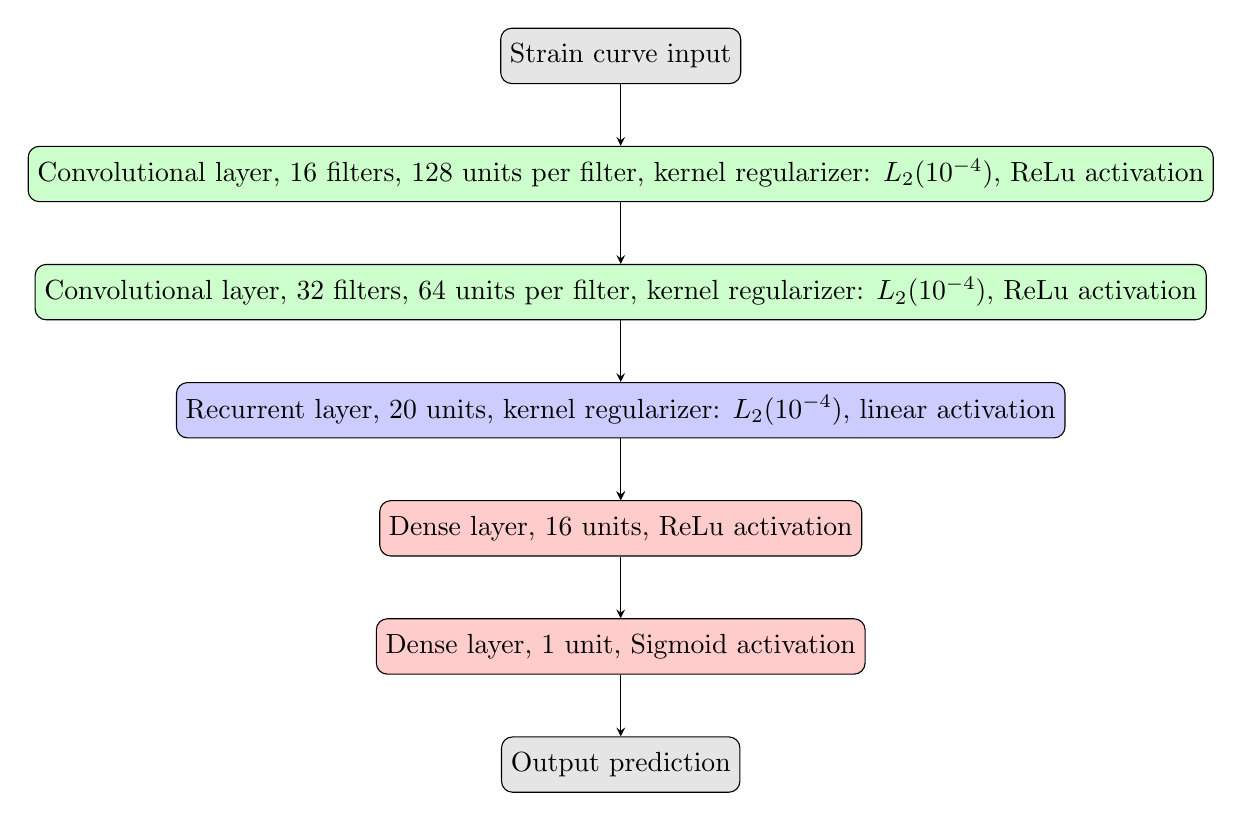
\begin{tikzpicture}
\node (input)  [io] {Strain curve input};
\node (conv1)  [conv,  node distance=1.5cm, below of=input]  {Convolutional layer, 16 filters, 128 units per filter, kernel regularizer: $L_2 (10^{-4})$, ReLu activation};
\node (conv2)  [conv,  node distance=1.5cm, below of=conv1]  {Convolutional layer, 32 filters, 64 units per filter, kernel regularizer: $L_2 (10^{-4})$, ReLu activation};
\node (lstm)   [lstm,  node distance=1.5cm, below of=conv2]  {Recurrent layer, 20 units, kernel regularizer: $L_2 (10^{-4})$, linear activation};
\node (dense1) [dense, node distance=1.5cm, below of=lstm]   {Dense layer, 16 units, ReLu activation};
\node (dense2) [dense, node distance=1.5cm, below of=dense1] {Dense layer, 1 unit, Sigmoid activation};
\node (output) [io,    node distance=1.5cm, below of=dense2] {Output prediction};

\draw [arrow] (input) --node {} (conv1);
\draw [arrow] (conv1) --node {} (conv2);
\draw [arrow] (conv2) --node {} (lstm);
\draw [arrow] (lstm) --node {} (dense1);
\draw [arrow] (lstm) --node {} (dense1);
\draw [arrow] (dense1) --node {} (dense2);
\draw [arrow] (dense2) --node {} (output);
\end{tikzpicture}

    \caption{A block diagram illustrating the architecture of the \acrshort{ann} used in this work.}
    \label{fig:nn_arch}
\end{figure}

\begin{table*}
    \centering
    \ra{1.3}
    \begin{tabular}{ llrr }
        \toprule
        Strain curves used                              & Views used  & Nr. of time series & Nr. of trainable parameters \\
        \midrule                                     
        \acrshort{gls}, or single \acrshort{rls} curves & Single view &         1          & 39,457 \\
        \acrshort{gls} curves                           &  All views  &         3          & 43,553 \\
        \acrshort{rls} curves                           & Single view &         6          & 49,697 \\
        \acrshort{rls} curves                           &  All views  &        18          & 74,273 \\
        \acrshort{gls} and \acrshort{rls} curves        & Single view &         7          & 51,745 \\
        \acrshort{gls} and \acrshort{rls} curves        &  All views  &        21          & 80,417 \\
        \bottomrule
    \end{tabular}
    \caption{This table shows the total number of trainable parameters of the \acrshort{ann}, for different number of time-series inputs.}
    \label{tab:train_params}
\end{table*}

Since the author did not design the architecture of the network, a thorough defence of the architecture will not be given. However, a brief explanation of the properties the different layers contribute with to the model as a whole will be given. The two first layers in the \acrshort{ann} are convolutional, and are intended to detect simple structures in the time series such as linear regions, curved regions and rapid changes in the signal. The recurrent layer is intended to detect time dependant relations of the signal such as periodicity and frequency. Regularization terms are added to the outputs of the convolutional, and recurrent layers to attempt to bias the weights toward zero, which is a technique used to avoid overfitting.Finally the dense layers are intended to connect the features extracted by the previous layers to specific values the target variable can have, and make a prediction.

\subsection{Training and Validation}

Binary cross entropy was used as loss function during training of the variations of the \acrshort{ann} model. Each variation was trained for five epochs, using back propagation and \acrshort{sgd}. The ADAM learning rate optimizer was used with an initial learning rate of $10^{-3}$ with the intention of avoiding that the loss function of the \acrshort{ann} got stuck in local minima during training. The baises of each layer were initialized as zeros, and the weights of the individual units were initialized by sampling from the standard normal distribution function. \bigskip. 

To validate the \acrshort{ann} models, 10-fold cross-validation was used. $N$-fold cross validation of a model-dataset combination entails dividing the dataset into N chunks of equal size, and preferably with an approximately equal distribution of target-variable values in each chunk. Then in N rounds, called \textit{folds} $N-1$ chunks are used to train the model and the final chunk is used to test the model. For each round one also changes which chunk is used to test the model such that it is able to attempt making a prediction on every value of the dataset. When validating the variations of the \acrshort{ann} using cross-validation the number of \acrshort{tp}, \acrshort{tn}, \acrshort{fp} and \acrshort{fn} attained during each fold were recorded and added together after all the folds were complete. The sum of all \acrshort{tp}, \acrshort{tn}, \acrshort{fp} and \acrshort{fn} attained during cross-validation are used to estimate the models' accuracy, sensitivity, specificity and DOR. Since there are a total of twelve datasets and three types of preprocessing tested, there are a total of 36 variations of the \acrshort{ann} model applied in the heart failure and patient diagnosis case studies. In the segment indication case study there is only one dataset, and three forms of preprocessing tested, so there are only three variations of the \acrshort{ann} model tested.

\section{Peak-value Supervised Classifiers} \label{sec:meth_pvsc}

Eleven base supervised classifiers are included in the \acrshort{pvsc} model group. In this section a short description of the theory behind these classifiers, and the hyperparameters used in this work will be given. The \acrshort{pvsc} models are validated using 10-fold cross-validation in the same manner as the \acrshort{ann} models.

\subsection*{Multi-layer Perceptron}
The \acrshort{mlp} is mentioned earlier described earlier in section \ref{sec:mlp}. This \acrshort{mlp} is configured with a single dense layer with a 100 neurons with the \acrshort{relu} activation, and an output layer of a single neuron since the classification problem is binary. It is trained with using \acrshort{sgd} with back-propagation, with ADAM as gradient descent optimizer, and an initial learning rate of $10^{-3}$.

\subsection*{K Nearest Neighbors}
\acrfull{knn} is an unbiased machine learning model that can be used for classification and for regression. When used for classification the target variable is predicted based on the points from the training set which are ''nearest'' in terms of input variable values. In the implementation used in this work, the model was constricted to only consider five closest neighbors weighted equally. 

\subsection*{Support Vector Classifier}
Support vector machines were originally implemented as a type of binary classifier that could classify linearly separable variables, as classifiers they are referred to as \acrfull{svc}. Under ideal conditions \acrshort{svc} transform input variables to a set of hyperplanes where the target variable values are linearly separable \cite{svm_wikipedia}. The transformation used depends on what kernel is used, some examples of kernel functions include: Linear kernal, \acrfull{rbf} and sigmoid function. In this work two versions of the \acrshort{svc} are tested, one with a linear kernel and one where the \acrshort{rbf} is used. The \acrshort{rbf} is given in in equation \eqref{eq:rbf}, where $\gamma$ is equal to 2. Both \acrshort{svc} applied use an $L_2$ regularization penalty to avoid overfitting. For the \acrshort{rbf} \acrshort{svc} parameter $C$ which is the inverse strength of the regularization is set to 1. For the linear \acrshort{svc} C is set to $0.025$.

\begin{equation}
    \mathrm{RBF}(\mathbf{x}) = e^{\gamma \left ( \mathbf{x} - \mathbf{c} \right )^2}
    \label{eq:rbf}
\end{equation}

\subsection*{Gaussian Process Classifier}
\acrshort{gp} are a probabilistic machine learning technique that can be used for regression, and classification tasks. Similar to \acrshort{svc} they perform best when the relationship between the input variables and the target variable are linear, but by the use of what is called \textit{basis functions} they can map the input variables to a hyperplane where the targets are linearly seperable \cite{GP_book}. One can say that basis functions are for \acrshort{gp}, what kernels are for \acrshort{svc}. The defining difference are that \acrshort{gp} are probabilistic while \acrshort{svc} are deterministic. Where \acrshort{svc} work with a single kernel \acrshort{gp} work with an infinite set of basis functions, and much of the training process amounts to finding an optimal linear combination of the set of kernals available \cite{GP_book}.

\subsection*{Decision Tree Classifiers}

\begin{itemize}
    \item Single decision tree
    \item Extra decision tree
    \item Random forest
\end{itemize}

Decision tree classifiers are classifiers that create hierarchies of rules that are used to make predictions of the target variable based on the values of the input variables \cite{scikit_learn}.

\subsection*{Ada boost classifier}

\subsection*{Naive Bayes Classifier}

\subsection*{Quadratic Discriminant Analysis}

\section{Presentation of Results}